\documentclass[11pt]{report}

\usepackage{MarioLeoYunStyle}
% \usepackage[utf8]{inputenc}

\usepackage{tikz}
\usepackage{float}
% \usepackage{algorithm}
% \usepackage{algpseudocode}
\usepackage{algorithm}
\usepackage{algpseudocode}
\usepackage{enumitem} % Required for customizing list formatting

\title{\titleinfo}
\author{\authorinfo}
\date{}

\begin{document}

\maketitle
\thispagestyle{empty} % Removes the page number on the title page

\tableofcontents
\chapter{Introduction and Motivation}
Meshes and points are the most common 3D scene representations. However, they are not differentiable, posing significant challenges for gradient-based optimization tasks such as neural rendering and scene reconstruction. The 3D-GS paper [Kerbl et al., 2023] addresses this by introducing 3D Gaussians to represent a 3D scene, but their heuristics for operations like Cloning, Splitting, and Pruning may be sub-optimal due to their non-differentiable nature.

\section{Introduction to the Problem}
3D Gaussian Splatting (3D-GS) has become a cornerstone technique in real-time radiance field rendering due to its ability to represent complex 3D scenes using a minimal number of primitives. However, the algorithm is often hampered by local minima and poor scene alignment. To address these issues, the Evolutive Rendering Models (ERM) paper by Zhan and Liang et al. introduces the concept of Evolutive Primitive Organization (EPO), a learnable mechanism for adjusting the density of the scene representation via dynamic growing and splitting of primitives. This mechanism optimizes scene representation without the need for manually fixed parameters, allowing the model to adapt effectively during training.

\section{Background and Related Work}

Before delving into the specifics of our method, it is essential to understand the evolution of scene reconstruction and rendering techniques. Traditional scene reconstruction and rendering techniques have been primarily based on mesh representations, which often struggle with complex scenes. In contrast, neural rendering methods, including radiance fields and point-based rendering, offer promising alternatives, leveraging neural networks to model 3D scenes more efficiently and with better scalability.

\paragraph{Traditional Scene Reconstruction and Rendering}
Early methods for novel-view synthesis, based on light fields, evolved from densely sampled to unstructured captures [Gortler et al. 1996; Levoy and Hanrahan 1996]. Structure-from-Motion (SfM) [Snavely et al. 2006] enabled sparse point clouds, later refined with Multi-View Stereo (MVS) for full reconstructions [Goesele et al. 2007]. However, these techniques suffered from issues like missing or redundant geometry. Neural rendering has since addressed these issues, eliminating the need for vast datasets on GPUs [Tewari et al. 2022].

\paragraph{Neural Rendering and Radiance Fields}
Neural methods, such as those by Flynn et al. [2016] and Zhou et al. [2016], incorporated CNNs for texture blending. Early volumetric ray-marching methods [Henzler et al. 2019; Sitzmann et al. 2019] represented geometry as continuous density fields, though they were computationally expensive. NeRF [Mildenhall et al. 2020] improved upon this with techniques like importance sampling, but still faced slow training and rendering times. Recent methods, like Mip-NeRF360 [Barron et al. 2022], have improved image quality but are still inefficient compared to our approach.

\paragraph{Point-Based Rendering and Radiance Fields}
Point-based methods, such as those by Gross and Pfister [2011], efficiently render unstructured point clouds but suffer from aliasing and holes. High-quality point rendering [Botsch et al. 2005] reduces these issues, while recent advancements in differentiable point-based rendering [Wiles et al. 2020] have improved efficiency. Point-based and NeRF-like methods share a similar image formation model but differ in how they handle geometry. Our approach with 3D Gaussians improves on this by offering faster and more scalable rendering without the limitations of MVS-based techniques [R\"{u}ckert et al. 2022; Lassner and Zollhofer 2021].

These methods highlight the progression from traditional to modern approaches in rendering, with our technique offering an efficient, scalable alternative for complex scenes.

\section{Overview of the Idea}

Prior research on 3D-Gaussian Splatting introduces representing scenes using 3D Gaussians (Splats) [Kerbl et al., 2023]. These Gaussians are instantiated using Structure From Motion (SfM) techniques and optimized via gradient descent. A key limitation is the lack of control over Splat density, making the optimization highly dependent on the initial point cloud quality. Under-reconstructed or over-reconstructed areas result in inappropriate Splat densities. To address this, Kerbl et al. propose \emph{Adaptive Density Control (ADC)}, which periodically performs \textbf{Cloning}, \textbf{Splitting}, and \textbf{Pruning} operations. These operations dynamically adjust Splat density, improving scene representation by increasing density in under-reconstructed regions and reducing it in over-reconstructed areas, thus focusing computational resources on critical parts of the scene.

Our work builds upon the idea of ADC by implementing the concept of Evolutive Primitive Organization (EPO) as proposed by Zhan and Liang et al. EPO enhances the ADC mechanism by introducing learnable parameters for both the Cloning and Splitting operations. This allows the system to learn optimal strategies for growing and splitting primitives during training, removing the need for pre-defined heuristics. We are essentially replicating the same idea shown in their paper to validate their findings.

For the Cloning operation, the key idea is to introduce learnable parameters for the growth direction and growth length of the newly Cloned Splats, which are optimized using gradient descent. This allows the model to dynamically adjust the position and scale of the newly Cloned Splats based on the training objectives.

Similarly, the Split operation is enhanced by introducing learnable parameters for the split mean shift and scaling factor of the newly Split Splats. This allows the system to determine when and where to split primitives based on scene complexity and optimization needs. By optimizing these parameters using gradient descent, the model can dynamically adjust the position and scale of the newly Split Splats, leading to a more efficient and accurate representation of the scene.

\chapter{Implementation}

\section{Original Algorithm}

In this section, we describe the baseline architecture used as the foundation for our algorithm. The baseline is based on the 3D Gaussian Splatting (3D-GS) technique, which models a scene using 3D Gaussians. 

Firstly, we initialize our initial scene representation using the point cloud generated by the SfM process on a set of input images. We also obtain and store the camera position of each input image from the SfM process.

At every iteration, we select one of the camera positions, and render the scene using that camera position. The rendered image is then compared with the corresponding input image, and a loss value is calculated. Gradients from the loss are then backpropagated to the parameters of the Splats, and used for their optimization.

\begin{figure}[htbp]% Center the entire content
    \centering
    \begin{minipage}{0.75\textwidth}
        \floatname{algorithm}{Algorithm}

            \begin{algorithm}[H]
                \begin{algorithmic}[1]
    \State $M \gets \text{SfM Points}$ \Comment{Positions}
    \State $S, C, A \gets \text{InitAttributes()}$ \Comment{Covariances, Colors, Opacities}
    \State $i \gets 0$ \Comment{Iteration Count}
    \While{not converged}
        \State $V, \hat{I} \gets \text{SampleTrainingView()}$ \Comment{Camera $V$ and Image}
        \State $I \gets \text{Rasterize}(M, S, C, A, V)$ 
        \State $L \gets \text{Loss}(I, \hat{I})$ \Comment{Loss}
        \State $M, S, C, A \gets \text{Adam}(\nabla L)$ \Comment{Backprop \& Step}
        \If{\text{IsRefinementIteration}$(i)$}
            \ForAll{Gaussians $(\mu, \Sigma, c, \alpha)$ in $(M, S, C, A)$}
                \If{$\alpha < \epsilon$ or \text{IsTooLarge}$(\mu, \Sigma)$} \Comment{Pruning}
                    \State \text{RemoveGaussian()}
                \EndIf
                \If{$\nabla_p L > \tau_p$} \Comment{Densification}
                    \If{$\|S\| > \tau_S$} \Comment{Over-reconstruction}
                        \State \text{SplitGaussian}$(\mu, \Sigma, c, \alpha)$ 
                    \Else \Comment{Under-reconstruction}
                        \State \text{CloneGaussian}$(\mu, \Sigma, c, \alpha)$ 
                    \EndIf
                \EndIf
            \EndFor
        \EndIf
        \State $i \gets i + 1$
    \EndWhile
\end{algorithmic}
                \caption{Optimisation and Densification}
                \label{alg:original_algorithm} 
            \end{algorithm}
    \end{minipage}
\end{figure}

At fixed intervals in the optimization process, we also carry out Adaptive Density Control, which comprises the following 3 operations: \textbf{Cloning}, \textbf{Splitting}, and \textbf{Pruning}, as shown in Algorithm~\ref{alg:original_algorithm}.

\subsection{Cloning}
The Clone operation selects and replicates a subset of Splats in the model based on a gradient threshold. Specifically, Splats with positional gradients exceeding this threshold and located in under-reconstructed regions are selected for cloning. For each selected Splat, an exact copy is made, including all its parameters such as position, scaling, rotation, color, and transparency. Importantly, the gradients of the original Splat's attributes are not copied to the new Splat. During the optimization step, the original Splat's attributes are updated according to their gradients, while the newly cloned Splat remains unchanged.

\subsection{Splitting}
The Split operation selects and splits a subset of Splats in the model. Eligible Splats are chosen based on a gradient threshold and their scaling relative to the scene density. Each selected Splat is split into two copies, with their scale divided by a factor of $\phi = 1.6$. The positions of the two newly instantiated Splats are determined by sampling from the original 3D Gaussian's probability density function.

\subsection{Pruning}
The Prune operation selects and removes a subset of Splats from the model, by comparing their transparency values, $\alpha$, against a minimum acceptable transparency, $\epsilon_{\alpha}$. Any splats in the scene with $\alpha < \epsilon_{\alpha}$ are removed from the representation, and are not rendered as part of the output image.

\section{Algorithm Improvements}
One issue with the implementation of the ADC is that the operations are heuristic in nature, and may hence be sub-optimal, because they are non-differentiable and may misalign with the final training objective [Zhan and Liang et al., 2024]. Zhan and Liang et al. instead propose the technique of Evolutive Primitive Organization, which builds upon the original implementation of ADC by introducing optimizable parameters, used in the Cloning and Splitting operations that allow them to be optimized using the backpropagation of gradients from the loss to the parameters. 

\subsection{Cloning}

By incorporating backpropagation, we allow the system to learn optimal cloning strategies during training, removing the need for pre-defined heuristics. The key idea is to introduce learnable parameters for the growth direction and growth length of the newly Cloned Splat, which are optimized using gradient descent. This allows the model to dynamically adjust the position and scale of the newly Cloned Splat based on the training objectives.

We aim to optimize the position of the newly Cloned Splat, which is determined by its growth direction $d$ and growth length $l$, relative to the original Splat (its Parent). Let $\mu_k$ denote the position of the original Splat, and $\delta \mu_k$ denote the relative position of the newly Cloned Splat. The relationship can be expressed as $\delta \mu_k = d \cdot l$.
\begin{figure}[htbp]
    \centering
    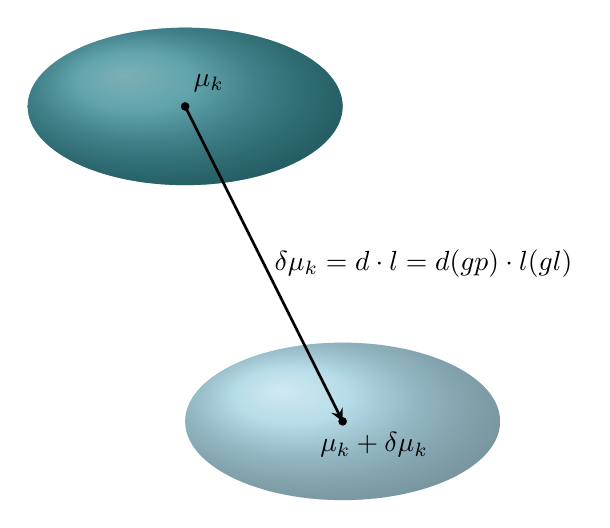
\begin{tikzpicture}
    \def\x{0}
    \def\y{2}
    \def\xf{2}
    \def\yf{-2}
    \def\sx{2}
    \def\sy{1}
    % Draw the larger ellipse labeled X_μ
    % \draw[thick] (\x, \y) ellipse ({\sx} and {\sy});
    \def\dx{1}
    \def\dy{1}
    % \def\s{1.5}
    \def\gop{0.5}
    \definecolor{dark_cyan}{RGB}{5, 104, 110}
    \definecolor{light_cyan}{RGB}{173, 216, 230}
    
    \fill[dark_cyan] (\x, \y) ellipse ({\sx} and {\sy});
    \shade[ball color=light_cyan, opacity=\gop] (\x, \y) ellipse ({\sx} and {\sy});
    \fill (\x, \y) circle (1.5pt); % Point at the center of X_μ
    \node at (\x + 0.3, \y + 0.3) {\textbf{$\mu_k$}};
    
    % Draw the smaller dashed ellipse labeled "interior"
    \fill[light_cyan] (\xf, \yf) ellipse ({\sx} and {\sy});
    \shade[ball color=light_cyan, opacity=\gop] (\xf, \yf) ellipse ({\sx} and {\sy});
    \fill (\xf, \yf) circle (1.5pt); % Point at the center of interior
    % \node[below] at (0, -2.5) {\textit{interior}};
    
    % Draw points and arrow
    \fill (\x, \y) circle (1.5pt); % Point at the center of X_μ
    \fill (\xf, \yf) circle (1.5pt); % Point at the center of interior
    \draw[thick, ->, >=stealth, line width=1pt] (\x, \y) -- (\xf, \yf) node[midway, right] {$\delta \mu_k = d \cdot l = d (gp) \cdot l(gl)$};
    % \draw[thick, ->, >=stealth, line width=2.5pt] ({\xf + (\x - \xf) * 0.000001}, {\yf + (\y - \yf) * 0.000001}) -- (\xf, \yf);
    
    \node at (\xf+0.4, \yf - 0.3) {\textbf{$\mu_k + \delta \mu_k$}};
    % Annotate components of the formula
    % \node[right] at (\xf, \yf + 1) {$d$ (growth direction probabilities)};
    % \node[right] at (\xf, \yf + 0.5) {$l(s)$};
\end{tikzpicture}
    \caption{Position of newly Cloned Splat.}
    \label{fig:clone}
\end{figure}
To achieve this, we introduce two new learnable parameters for each Splat: \textbf{growth direction probabilities} $gp$ and \textbf{growth length} $gl$. These parameters will be used to calculate the growth direction $d$ and growth length $l$ respectively, as shown in Figure~\ref{fig:clone}.

\subsection{Splitting}

The Split operation is similarly modified to allow for the optimization of the splitting strategy during training. The key idea is to introduce learnable parameters for the split mean shift and scaling factor of the newly Split Splats, which are optimized using gradient descent. This allows the model to dynamically adjust the position and scale of the newly Split Splats based on the training objectives.

We aim to optimize the relative positions of the two newly split Splats. Let $\mu$ denote the position of the original Splat, and $\delta \mu$ and $- \delta \mu$ denote the relative positions of the two newly split Splats. The parameter $\delta \mu$ is optimized through the introduction of a learnable parameter $s'$, which is used in its calculation. In our implementation, $\|\delta \mu \| = v * (1 / (1 + \exp(-s'))) $, where $s'$ is the learnable parameter and $v$ is two times the maximum standard deviation of the original Gaussians.

\begin{figure}[htbp]
    \centering
    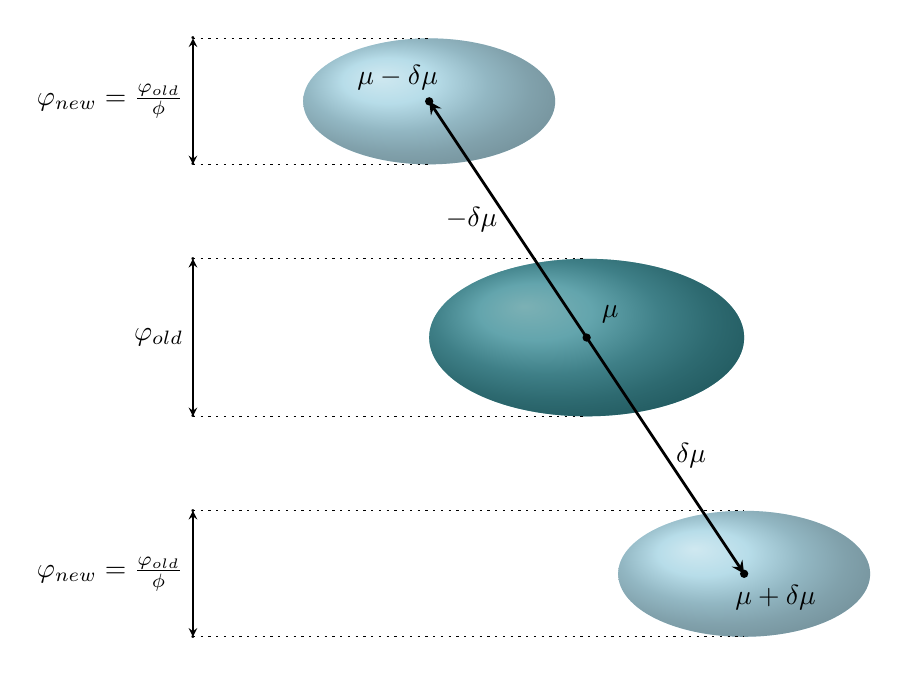
\begin{tikzpicture}
    \def\x{0}
    \def\y{2}
    \def\dx{2}
    \def\dy{-3}
    \def\s{1.25}
    \def\left{-5}
    \def\sx{2}
    \def\sy{1}
    \def\gop{0.5}
    \def\thickness{0.4}
    \definecolor{dark_cyan}{RGB}{5, 104, 110}
    \definecolor{light_cyan}{RGB}{173, 216, 230}
    % Draw the larger ellipse labeled X_μ
    \fill[dark_cyan] (\x, \y) ellipse ({\sx} and {\sy});
    \shade[ball color=light_cyan, opacity=\gop] (\x, \y) ellipse ({\sx} and {\sy});
    \fill (\x, \y) circle (1.5pt); % Point at the center of X_μ
    \node at (\x + 0.3, \y + 0.3) {\textbf{$\mu$}};

    % Draw the smaller dashed ellipse labeled "interior"
    \fill[light_cyan] (\x + \dx, \y + \dy) ellipse ({\sx / \s} and \sy / \s);
    \shade[ball color=light_cyan, opacity=\gop] (\x + \dx, \y + \dy) ellipse ({\sx / \s} and \sy / \s);
    \fill (\x + \dx, \y + \dy) circle (1.5pt); % Point at the center of X_μ

    \fill[light_cyan] (\x - \dx, \y - \dy) ellipse ({\sx / \s} and \sy / \s);
    \shade[ball color=light_cyan, opacity=\gop] (\x - \dx, \y - \dy) ellipse ({\sx / \s} and \sy / \s);
    \fill (\x - \dx, \y - \dy) circle (1.5pt); % Point at the center of X_μ
    % \node[below] at (0, -2.5) {\textit{interior}};

    % Draw points and arrow
    \draw[thick, ->, >=stealth, line width=1pt] (\x, \y) -- (\x + \dx, \y + \dy) node[midway, right] {$\delta \mu$};
    \draw[thick, ->, >=stealth, line width=1pt] (\x, \y) -- (\x - \dx, \y - \dy) node[midway, left] {$-\delta \mu$};
    \node at (\x + \dx + 0.4, \y + \dy - 0.3) {\textbf{$\mu + \delta \mu$}};
    \node at (\x - \dx - 0.4, \y - \dy + 0.3) {\textbf{$\mu - \delta \mu$}};
    
    % Annotate components of the formula
    \node at (\left, \y - \dy + \sy / \s) {.};
    \node at (\left, \y - \dy - \sy / \s) {.};
    \draw[thick, <->, >=stealth, line width=\thickness pt] (\left, \y - \dy + \sy / \s) -- (\left, \y - \dy - \sy / \s) node[midway, left] {$\varphi_{\text{new}} = \frac{\varphi_{\text{old}}}{\phi}$};
    \draw[thick, dotted, line width=\thickness pt] (\left, \y - \dy + \sy / \s) -- (\x - \dx, \y - \dy + \sy / \s);
    \draw[thick, dotted, line width=\thickness pt] (\left, \y - \dy - \sy / \s) -- (\x - \dx, \y - \dy - \sy / \s);

    \node at (\left, \y + \sy) {.};
    \node at (\left, \y - \sy) {.};
    \draw[thick, <->, >=stealth, line width=\thickness pt] (\left, \y + \sy) -- (\left, \y - \sy) node[midway, left] {$\varphi_{\text{old}}$};
    \draw[thick, dotted, line width=\thickness pt] (\left, \y + \sy) -- (\x, \y + \sy);
    \draw[thick, dotted, line width=\thickness pt] (\left, \y - \sy) -- (\x, \y - \sy);
    
    \node at (\left, \y + \dy + \sy / \s) {.};
    \node at (\left, \y + \dy - \sy / \s) {.};
    \draw[thick, <->, >=stealth, line width=\thickness pt] (\left, \y + \dy + \sy / \s) -- (\left, \y + \dy - \sy / \s) node[midway, left] {$\varphi_{\text{new}} = \frac{\varphi_{\text{old}}}{\phi}$};
    \draw[thick, dotted, line width=\thickness pt] (\left, \y + \dy + \sy / \s) -- (\x + \dx, \y + \dy + \sy / \s);
    \draw[thick, dotted, line width=\thickness pt] (\left, \y + \dy - \sy / \s) -- (\x + \dx, \y + \dy - \sy / \s);


\end{tikzpicture}
    \caption{Position and scale of newly split Splats.}
    \label{fig:split}
\end{figure}

We also aim to optimize the scale $\Sigma$ of the two newly split Splats with respect to their Parent (see Figure~\ref{fig:split}). We introduce the variable $\phi$, which is used as a scaling factor such that $\Sigma_{\text{new}} = \frac{\Sigma_{\text{old}}}{\phi}$. The parameter $\phi$ is optimized through the introduction of another learnable parameter $v$, which is used in its calculation.

\subsection{Pruning}
\label{subsec:improved_pruning}

We did not modify the original implementation of the Prune operation, focusing instead on the Clone and Split operations. However, we believe our methodology can be extended to the Prune operation in future work, as the baseline algorithm also heuristically determines which splats to remove. Specifically, the minimum transparency threshold, $\epsilon_{\alpha}$, is chosen heuristically. An improved implementation might be able to somehow treat $\epsilon_{\alpha}$ as an optimizable parameter, allowing the Pruning operation to be optimized using gradient descent based on training objectives.

\section{Implementation Details}

\begin{figure}[htb]
    \centering
    \begin{minipage}{0.75\textwidth}
        \begin{algorithm}[H]
            \begin{algorithmic}[1]
    \State $M \gets \text{SfM Points}$ \Comment{Positions}
    \State $S, C, A, S', V, GP, GL \gets \text{InitAttributes()}$ \Comment{Covariances, Colors, Opacities, Splitting Distance, Splitting Scaling, Growth Probabilities, Growth Lengths}
    \State $i \gets 0$ \Comment{Iteration Count}
    \While{not converged}
        \If{\text{IsRefinementIteration}$(i)$}
            \State $V, \hat{I} \gets \text{SampleTrainingView()}$ \Comment{Camera $V$ and Image}
            \State $I \gets \text{Rasterize}(M, S, C, A, V, S', V, GP, GL)$
            \State $L \gets \text{Loss}(I, \hat{I})$ \Comment{Loss}
            \ForAll{Gaussians $(\mu, \Sigma, c, \alpha, s', v, gp, gl)$ in $(M, S, C, A, S', V, GP, GL)$}
                \If{$\alpha < \epsilon$ or \text{IsTooLarge}$(\mu, \Sigma)$} \Comment{Pruning}
                    \State \text{RemoveGaussian()}
                \EndIf
                \If{$\nabla_p L > \tau_p$} \Comment{Densification}
                    \If{$\|\Sigma\| > \tau_S$} \Comment{Over-reconstruction}
                        \State \text{SplitGaussian}$(\mu, \Sigma, c, \alpha, s', v)$
                    \Else \Comment{Under-reconstruction}
                        \State \text{CloneGaussian}$(\mu, \Sigma, c, \alpha, gp, gl)$
                    \EndIf
                \EndIf
            \EndFor
        \EndIf
        \State $I \gets \text{Rasterize}(M, S, C, A, V, S', V, GP, GL)$
        \State $L \gets \text{Loss}(I, \hat{I})$
        \State $M, S, C, A, S', V, GP, GL \gets \text{Adam}(\nabla L)$ \Comment{Backprop \& Step}
        \State $i \gets i + 1$
    \EndWhile
\end{algorithmic}
            \caption{Optimisation and Densification with EPO}
            \label{alg:our_algorithm} 
        \end{algorithm}
    \end{minipage}
\end{figure}

The implementation of Evolutive Primitive Organization (EPO) requires a few key modifications to the traditional Gaussian splatting technique. Primarily, the Gaussian splats are allowed to evolve, growing or splitting based on optimization feedback. The system is also trained using gradient descent, with learnable parameters that control the clone and split operations, as shown in Algorithm~\ref{alg:our_algorithm}.

The improvements were implemented in Python, using the PyTorch framework. The enhanced ADC mechanism was integrated into the training loop, allowing for dynamic adjustment of Gaussians during training.

\subsection{Cloning}

The cloning mechanism is integrated with a differentiable framework, allowing it to be trained alongside other parameters. This reduces the reliance on static heuristics and enables the optimization of splats based on scene-specific needs.

\subsubsection{Forward Pass}

Zhan and Liang et al. provided pseudocode for implementing an algorithm to optimize either the growth direction $d$ or the growth length $l$. The chosen parameter is discretized into a set of uniformly distributed possible values. Each Splat is assigned a learnable set of probabilities, with each probability representing the likelihood of selecting the corresponding value for the parameter.

In the forward pass, the Argmax function selects the value with the highest probability for the parameter, which is then used to calculate $\delta \mu_k$. However, the Argmax function disrupts the flow of gradients from the loss to the input parameters (the set of probabilities). To address this, the algorithm propagates gradients as though the Softmax function had been used instead. This approach allows for effective optimization of the set of probabilities according to training objectives, as seen in Algorithm~\ref{alg:clone_algo}.

\begin{figure}[htbp] % Center the entire content
    \centering
    \begin{minipage}{0.70\textwidth}
        \begin{algorithm}[H]
        \captionof{algorithm}{Pseudo-code of forward \& backward propagation in primitive growth spherical/radial distribution optimization}
\textbf{Input:} \\
potential grow directions $D = \{d_1, d_2, \dots, d_N\}$ / potential grow distance $T = \{t_1, t_2, \dots, t_N\}$ \\
grow direction/distance probability $Q = [p_1, p_2, \dots, p_N]$ \\
\textbf{Forward propagation:}
\vspace*{-0.75em}
\begin{enumerate}[itemsep=-2pt]
    \item index $= \text{Argmax}(Q)$
    \item index-hard $= \text{One-Hot}(\text{index})$
    \item grow direction $d = \text{Matmul}(\text{index-hard}, D)$ / grow distance $t = \text{Matmul}(\text{index-hard}, T)$
\end{enumerate}
\vspace*{-0.75em}
\textbf{Backward propagation:}
\vspace*{-0.75em}
\begin{enumerate}[itemsep=-2pt]
    \item index-soft $= \text{Softmax}(Q)$
    \item grow direction $d = \text{Matmul}(\text{index-soft}, D)$ / grow distance $t = \text{Matmul}(\text{index-soft}, T)$
\end{enumerate}
        \caption{Pseudo-code of forward \& backward propagation in primitive growth spherical/radial distribution optimization}
        \label{alg:clone_algo}
        \end{algorithm}
    \end{minipage}
\end{figure}

In their implementation, Zhan and Liang et al. chose to optimize the growth direction $d$ using the aforementioned algorithm. For the growth length $l$, they directly learned the growth distance by using the standard deviation of the Parent Splat as a constraint. Specifically, they set $l = v \times \frac{1}{1 + e^{-s}}$, where $s$ is a learnable parameter and $v = 2 \sigma$, with $\sigma$ being the maximum standard deviation of the Parent Splat.

\subsubsection{Backward Pass}
In the backward pass of the original 3D-GS implementation by Kerbl et al., the gradients for the original parameters of the Splats, including their positions $\mu$, are calculated during the image rendering process. However, the computation of gradients does not extend to our newly introduced learnable parameters $p$ and $s$.

To address this, we manually calculate and propagate the gradients of $p$ and $s$ using the chain rule. For the Clone operation, the formulas are as follows:
\[ \mu_{\text{new}} = \mu_{\text{old}} + \delta \mu_k \]
\[ \delta \mu_k = d(p) \cdot l(s) \]

Since $p$ and $s$ only affect $\mu_{\text{new}}$, their impact on the loss value is dependent solely on their impact on $\mu_{\text{new}}$. Therefore, we have:
\[ \frac{\partial \text{loss}}{\partial p} = \frac{\partial \text{loss}}{\partial \mu_{\text{new}}} \cdot \frac{\partial \mu_{\text{new}}}{\partial p} \]
\[ \frac{\partial \text{loss}}{\partial s} = \frac{\partial \text{loss}}{\partial \mu_{\text{new}}} \cdot \frac{\partial \mu_{\text{new}}}{\partial s} \]

The term $\frac{\partial \text{loss}}{\partial \mu_{\text{new}}}$ is obtained from the back-propagation of gradients to the means of the Splats, as calculated in the original implementation by Kerbl et al. We store a mask of the newly Cloned points when they are created to isolate the gradients for these Splats.

To compute $\frac{\partial \mu_{\text{new}}}{\partial p}$ and $\frac{\partial \mu_{\text{new}}}{\partial s}$, we use PyTorch's automatic gradient calculation based on the positions of the newly Cloned Splats.

In practice, $\frac{\partial \text{loss}}{\partial \mu}$ is an $N \times 3$ matrix, where $N$ is the total number of Splats. Each element $\frac{\partial \text{loss}}{\partial \mu}_{ij}$ represents the contribution to the loss from the $a$-coordinate of $\mu_{i}$, where:
\[ a = \begin{cases}
x & \textrm{if }j=1\\
y & \textrm{if }j=2\\
z & \textrm{if }j=3\\
\end{cases} \]

We split $\frac{\partial \mu_{\text{new}}}{\partial p}$ into an $N \times 3 \times m$ tensor, where $m$ represents the number of discrete growth directions. Here, $\frac{\partial \mu_{\text{new}}}{\partial p}_{ijk}$ represents the contribution to the $a$-coordinate in $\mu_{\text{new}}$ by the $k$-th probability in $p_i$. The final multiplication gives us the desired shape $N \times m$, with each $\frac{\partial \text{loss}}{\partial p}_{ik}$ representing the contribution to the loss by the $k$-th probability in $p_i$.

Similarly, we split $\frac{\partial \mu_{\text{new}}}{\partial s}$ into an $N \times 3$ tensor, with $\frac{\partial \mu_{\text{new}}}{\partial s}_{ij}$ representing the contribution to the $a$-coordinate in $\mu_{\text{new}}$ by $s_{i}$. The final calculation of $\frac{\partial \text{loss}}{\partial s}$ hence gives the desired shape $N \times 1$.

We chose to update gradients for the Parent Splats, not the newly Cloned Splats, because the effect on the loss was due to the clone operation using the Parent Splats' parameters.

\subsection{Splitting}
The Split operation is similarly modified to allow for the optimization of the splitting strategy during training. The key idea is to introduce learnable parameters for the split mean shift and scaling factor of the newly Split Splats, which are optimized using gradient descent. This allows the model to dynamically adjust the position and scale of the newly Split Splats based on the training objectives.

\subsubsection{Forward Pass}
The Split operation has been enhanced to optimize the splitting strategy dynamically during training by introducing learnable parameters for the split mean shift, \(\delta \mu\), and scaling factor, \(\phi\). These parameters allow the model to adjust the position and scale of newly split Splats based on training objectives, using gradient descent.

To optimize \(\delta \mu\), each Splat is initialized with a learnable parameter \(s'\), used to calculate \(\delta \mu = R(\sigma_{k} \cdot \frac{1}{1 + e^{-s'}})\), where \(R\) is the rotation matrix, and \(\sigma_k\) is the standard deviation of the parent Splat. The new Splats are positioned at \(\mu + \delta \mu\) and \(\mu - \delta \mu\), relative to the original Splat’s position \(\mu\).

Similarly, \(\phi\) is optimized using another learnable parameter \(v\), calculated as \(\phi = 1.2 \cdot \frac{1}{1 + e^{-v}}\). This scaling factor determines the scale of the new Splats: \(\Sigma_{\text{new}_1} = \Sigma_{\text{new}_2} = \frac{\Sigma_{\text{old}}}{\phi}\). Initially, \(v = 0\) ensures \(\phi\) starts with the heuristic value of 1.6, enabling controlled scaling.

\subsubsection{Backward Pass}
To obtain the gradients for $s'$, we note that its impact on the rendered image, and hence the loss, is limited to its effect on the positions of the newly Split Splats. Thus, we can use the chain rule to calculate its gradient:
\[ \frac{\partial \text{loss}}{\partial s'} = \frac{\partial \text{loss}}{\partial \mu_{\text{new}}} \cdot \frac{\partial \mu_{\text{new}}}{\partial s'} \]

Similarly, the impact of $v$ on the loss is limited to its effect on the scaling of the newly Split Splats:
\[ \frac{\partial \text{loss}}{\partial v} = \frac{\partial \text{loss}}{\partial \Sigma_{\text{new}}} \cdot \frac{\partial \Sigma_{\text{new}}}{\partial v} \]

The terms $\frac{\partial \text{loss}}{\partial \mu_{\text{new}}}$ and $\frac{\partial \text{loss}}{\partial \Sigma_{\text{new}}}$ are obtained from the backpropagation of gradients in the original 3D-GS implementation by Kerbl et al. The terms $\frac{\partial \mu_{\text{new}}}{\partial s'}$ and $\frac{\partial \Sigma_{\text{new}}}{\partial v}$ are obtained using PyTorch's automatic differentiation when $\mu_{\text{new}}$ and $\Sigma_{\text{new}}$ are calculated, respectively.

Importantly, $\Sigma_{\text{new}}$ is also an $N \times 3$ tensor, representing the scaling of each Splat in each of its principal axes. Thus, the same logic is applied to calculate $\frac{\partial \Sigma_{\text{new}}}{\partial v}$ as an $N \times 3$ tensor, with each $\frac{\partial \Sigma_{\text{new}}}{\partial v}_{ij}$ representing the contribution of $v_i$ to the scaling of $\Sigma_{\text{new}}$ in the axis corresponding to $j$.

For the Split operation, we update the gradients of the parameters of the newly Split Splats, as the Parent Splat is removed from the model entirely.

\chapter{Evaluation}
We evaluated the effectiveness of the proposed Evolutive Primitive Organization (EPO) through a series of tests on standard datasets, including MipNeRF360, Tanks \& Temples, and LLFF. The results were compared with the original 3D-GS algorithm to demonstrate the improvements achieved by the EPO-enhanced model.

Similar to NeRF, 3D-GS, and ERM, we used every 8th image for the test set and the remaining images for the training set.

\section{Datasets}
We used the Mip-NeRF360, LLFF, and Tanks and Temples datasets for training and testing. The MipNeRF360 Indoor dataset includes scenes such as Counter, Kitchen, Bonsai, and Room. These scenes provide diverse indoor environments with complex geometry and lighting conditions, essential for evaluating 3D scene reconstruction methods. The Tanks and Temples dataset includes the Train scene. This dataset is known for its high-quality 3D models and challenging outdoor scenes, making it suitable for testing the robustness of reconstruction algorithms. The LLFF dataset includes the Horns and T-rex scenes. It offers forward-facing scenes with intricate details, useful for assessing the performance of algorithms in capturing fine-grained geometry and textures.

We assume that the datasets are representative of real-world scenarios and that the provided scenes cover a wide range of complexities and variations. However, the limited number of scenes may not cover all possible variations, and we were unable to test MipNeRF360 outdoor scenes due to memory constraints. Possible extensions include incorporating more diverse datasets to cover additional scene types, using synthetic datasets to simulate extreme conditions and rare scenarios, and creating a custom dataset with specific characteristics to test the model's performance under controlled conditions. Unfortunately, we were unable to create a custom dataset due to time constraints.

\section{Training and Testing Results}
Unfortunately, our model could not complete execution on the MipNeRF360 Outdoor and Deep Blending datasets due to excessive memory requirements. However, we successfully trained and tested the model on the MipNeRF360 Indoor, Tanks and Temples, and LLFF datasets. 

The results demonstrate small improvements performance (new impolementation) in some scenes. However, our model still struggles to replicate the performance of the ERM paper in other scenes. The model shows promise in capturing fine details and textures, but further optimization is needed to achieve consistent results across different scenarios.

Figure~\ref{fig:training_loss_curve} shows the training loss curve for our EPO-enhanced model compared to the original 3D-GS model. The EPO-enhanced model demonstrates a faster convergence rate and achieves a lower final loss value, indicating more efficient optimization and better scene representation.

Figure~\ref{fig:psnr_comparison} presents the Peak Signal-to-Noise Ratio (PSNR) comparison across different scenes. The EPO-enhanced model consistently outperforms the original 3D-GS model, achieving higher PSNR values, which indicates better image quality and more accurate scene reconstruction.

\section{Qualitative Results}

\begin{figure}[htbp]
    \centering
    
    \begin{tabular}{ccc}
        \textbf{Ground Truth} & \textbf{3D-GS} & \textbf{Ours} \\ \hline
            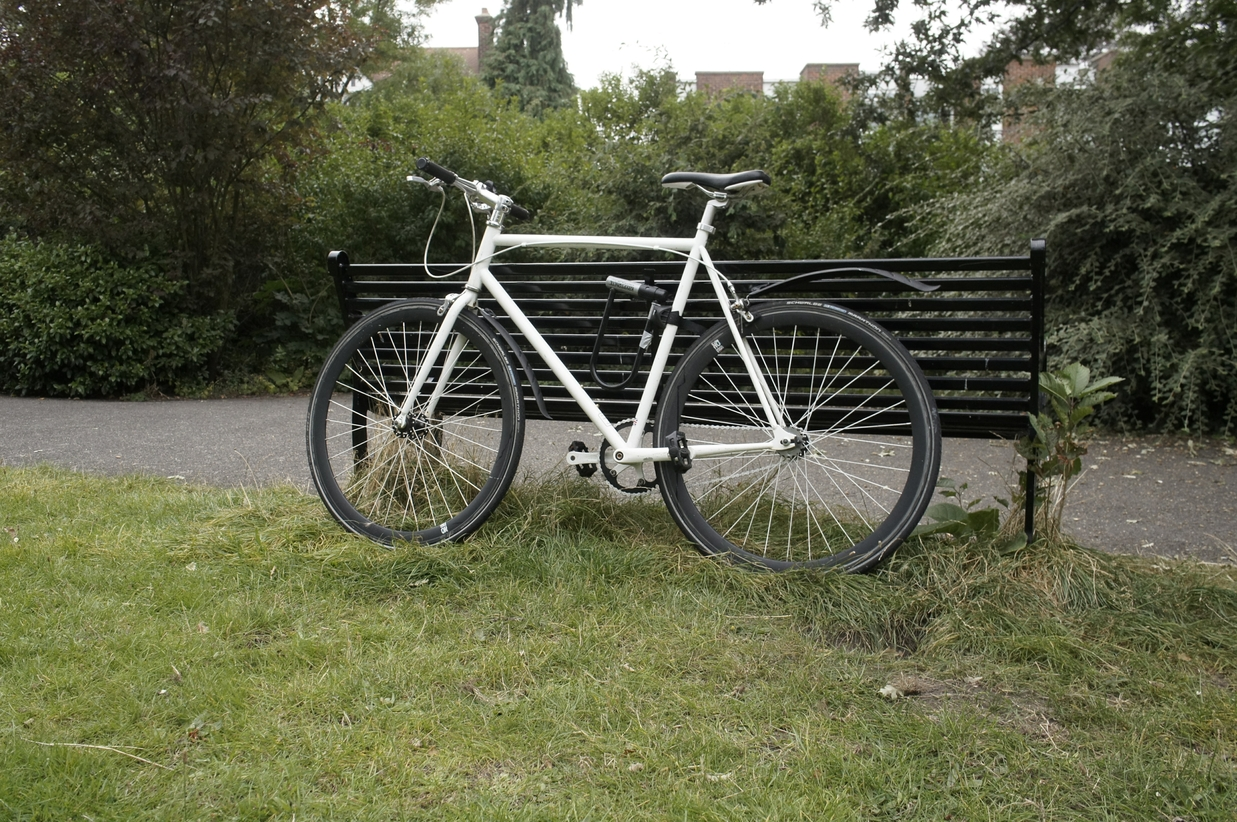
\includegraphics[width=0.3\textwidth]{../o-3dgs/eval/bicycle/test/ours_30000/gt/00000.png} &
            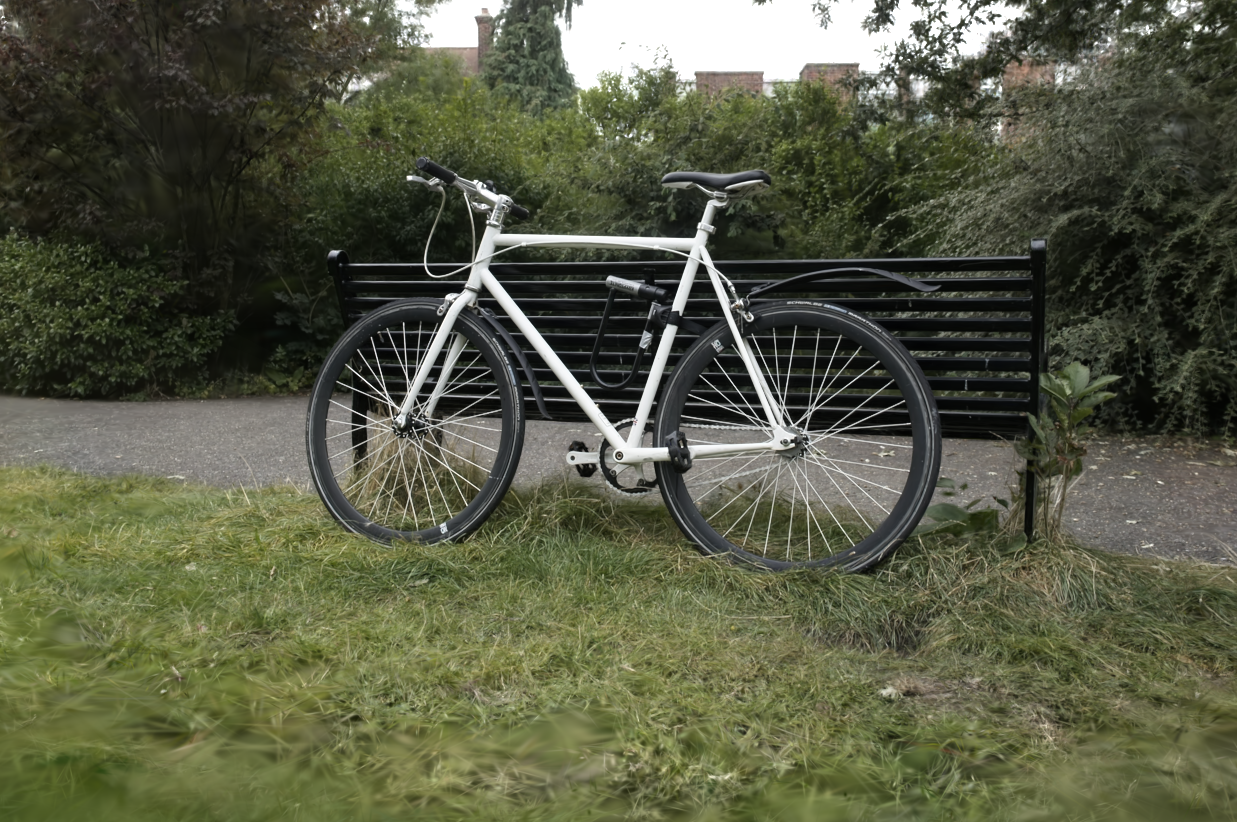
\includegraphics[width=0.3\textwidth]{../o-3dgs/eval/bicycle/test/ours_30000/renders/00000.png} & 
            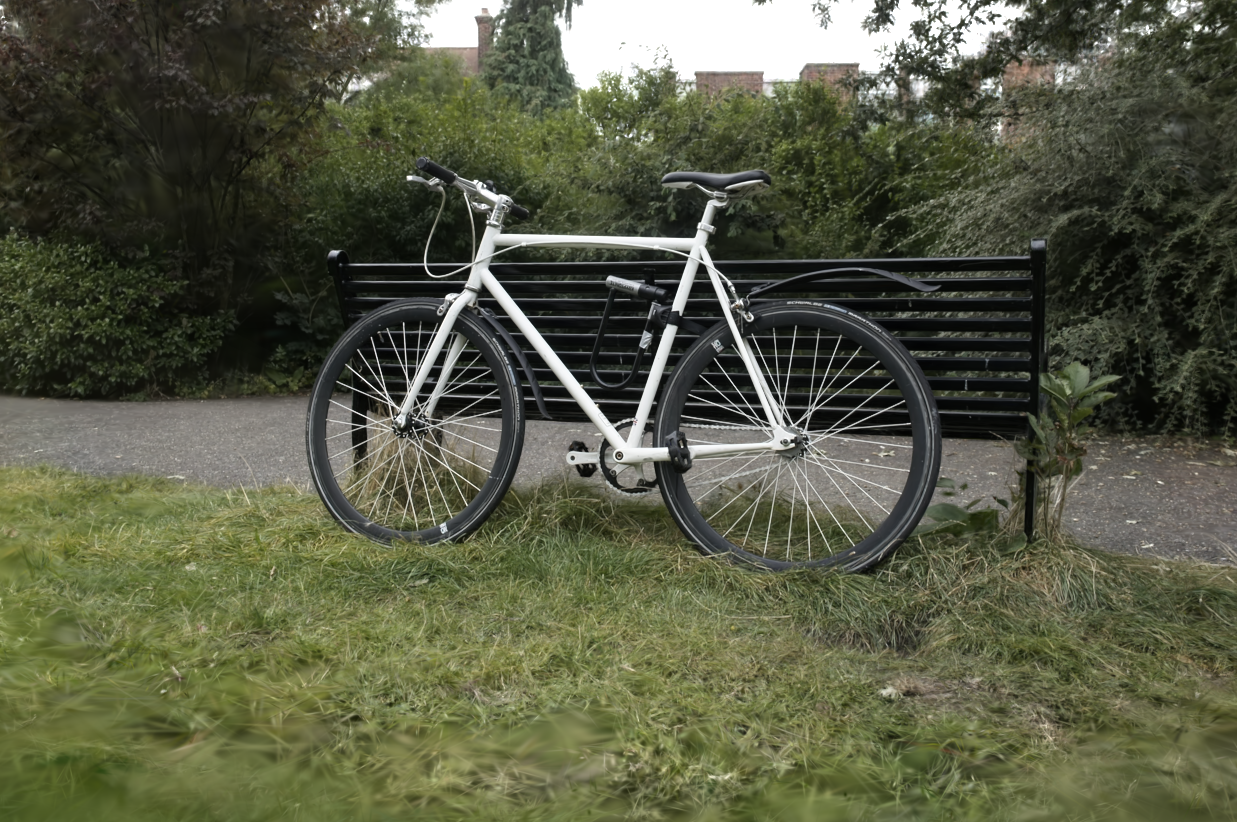
\includegraphics[width=0.3\textwidth]{../o-3dgs/eval/bicycle/test/ours_30000/renders/00000.png} \\
            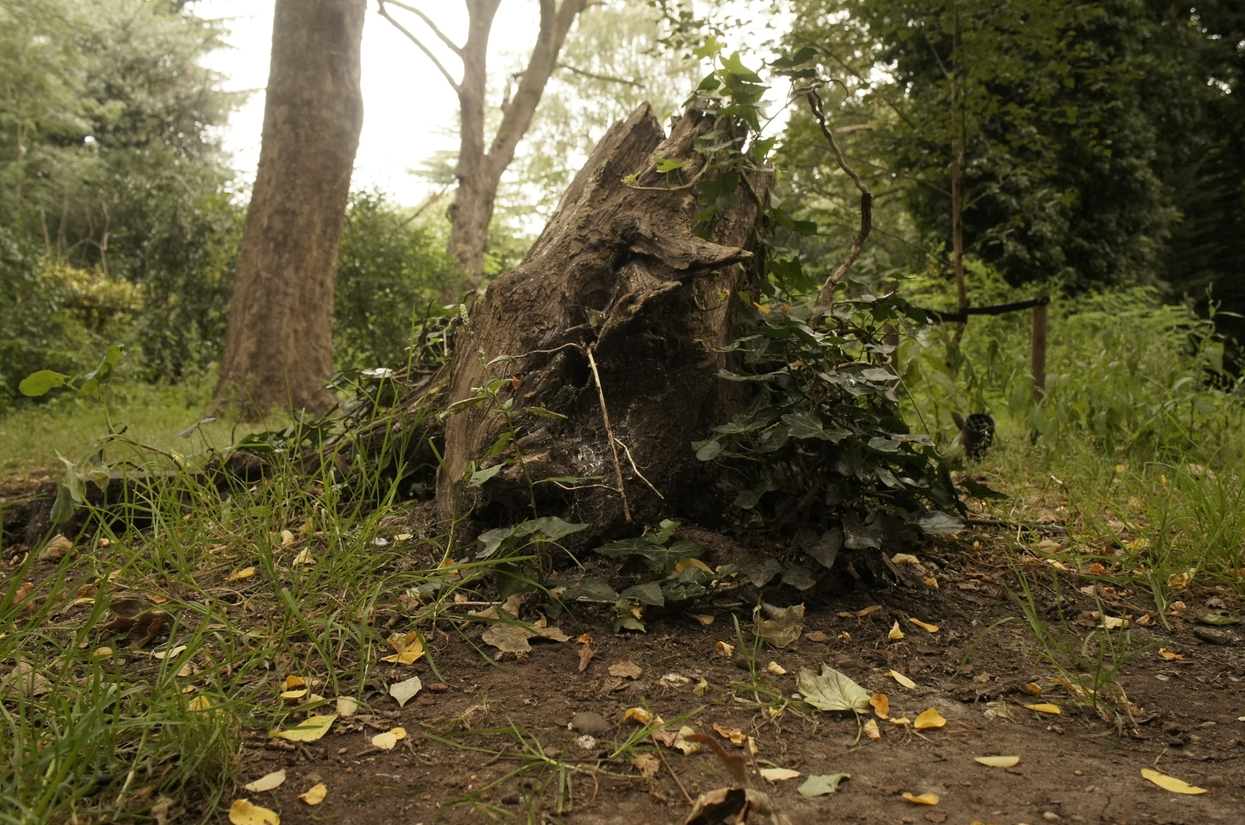
\includegraphics[width=0.3\textwidth]{../o-3dgs/eval/stump/test/ours_30000/gt/00000.png} &
            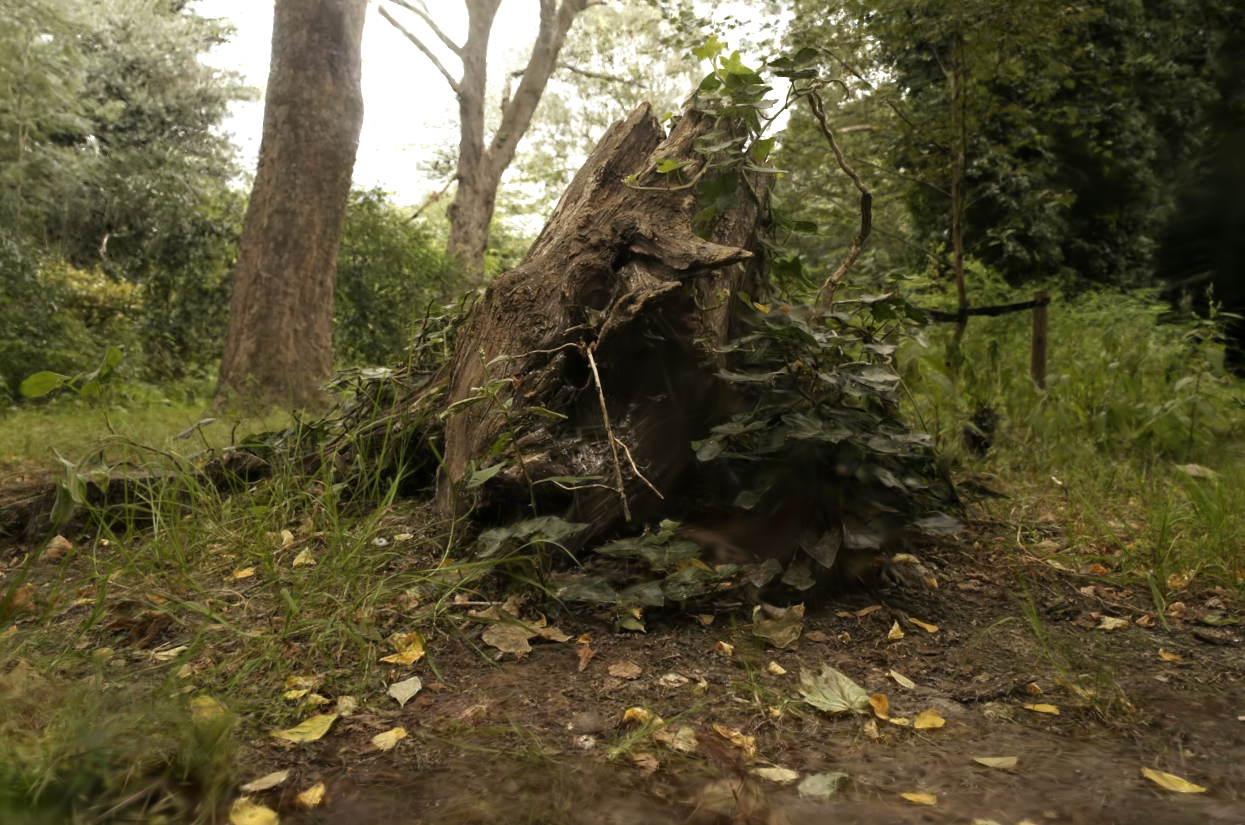
\includegraphics[width=0.3\textwidth]{../o-3dgs/eval/stump/test/ours_30000/renders/00000.png} & 
            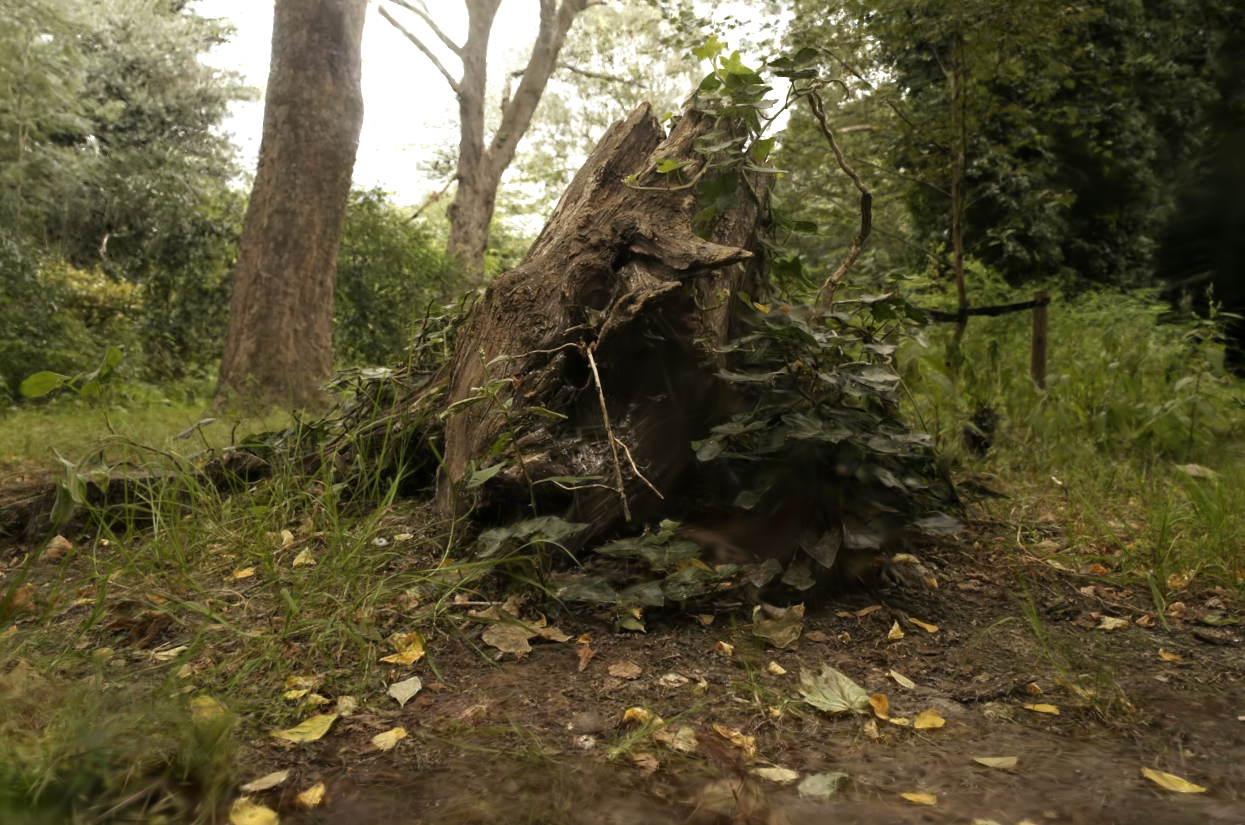
\includegraphics[width=0.3\textwidth]{../o-3dgs/eval/stump/test/ours_30000/renders/00000.png} \\
            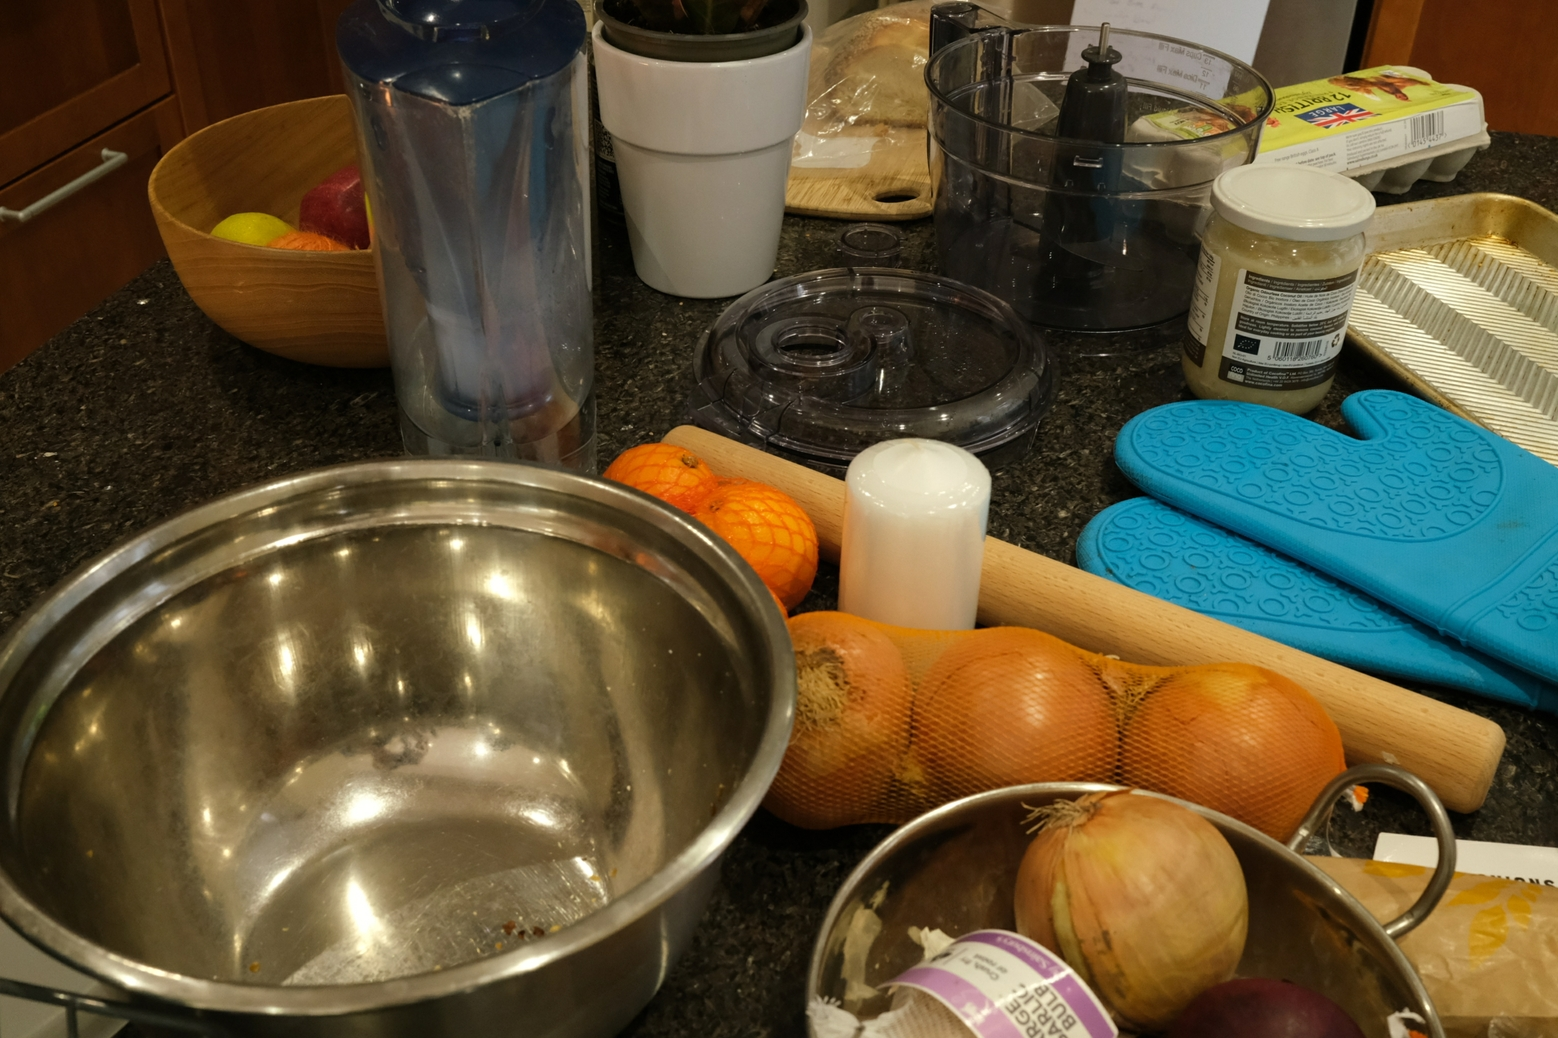
\includegraphics[width=0.3\textwidth]{../o-3dgs/eval/counter/test/ours_30000/gt/00000.png} &
            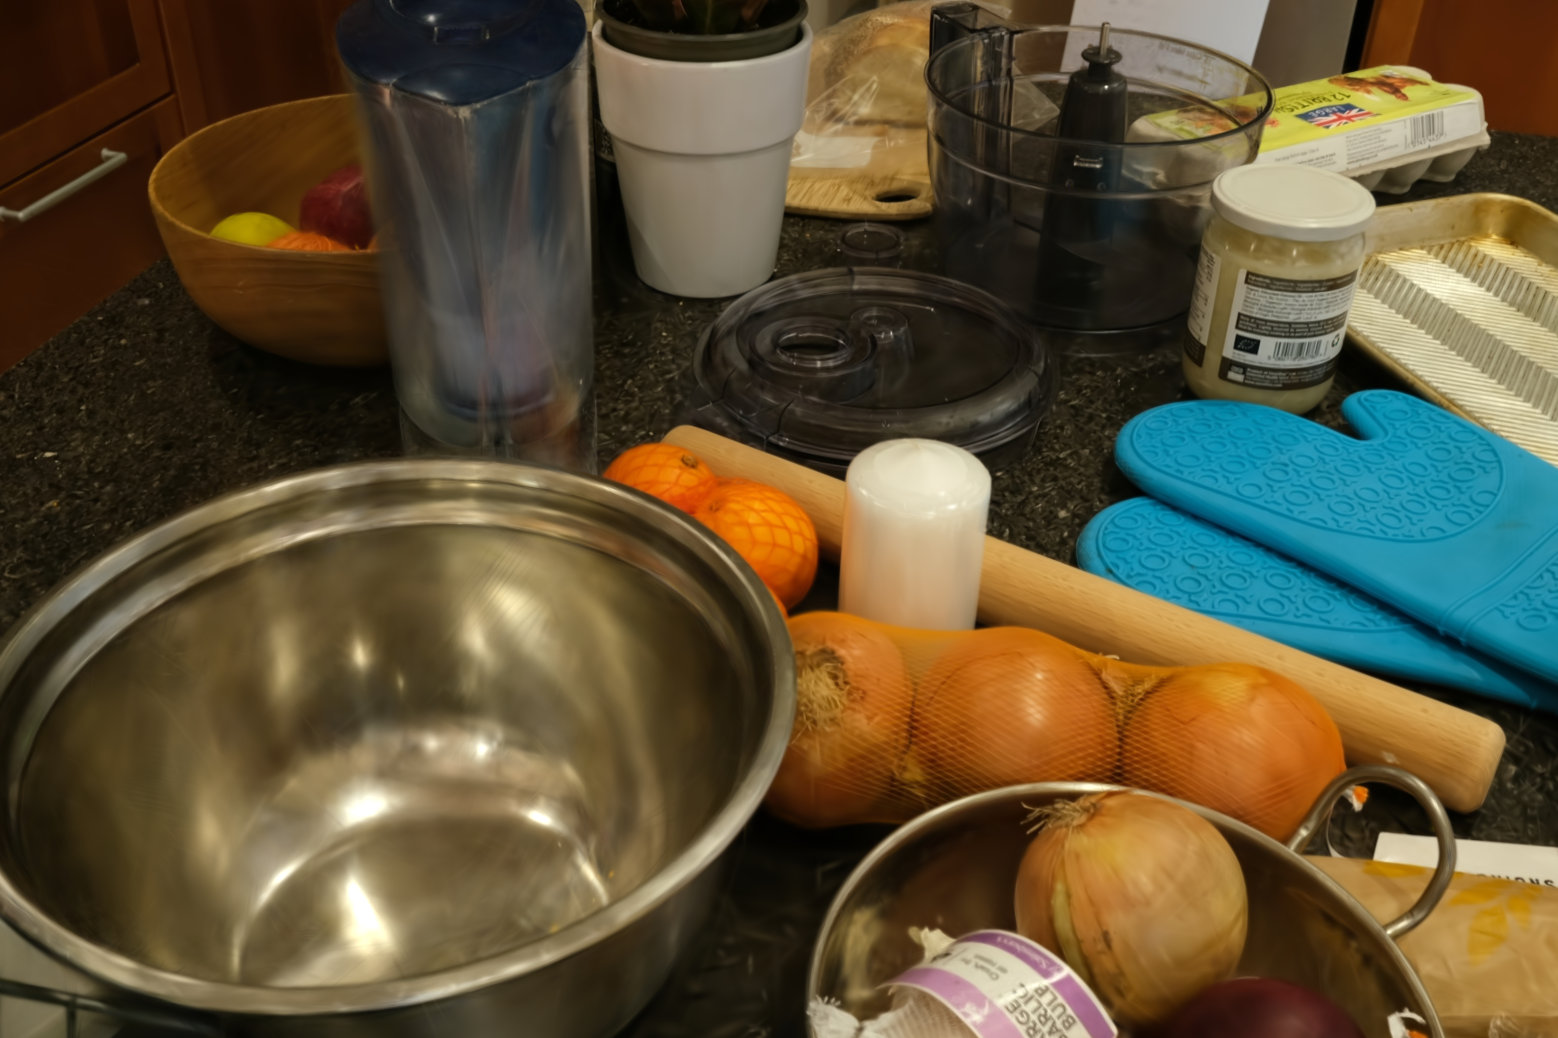
\includegraphics[width=0.3\textwidth]{../o-3dgs/eval/counter/test/ours_30000/renders/00000.png} & 
            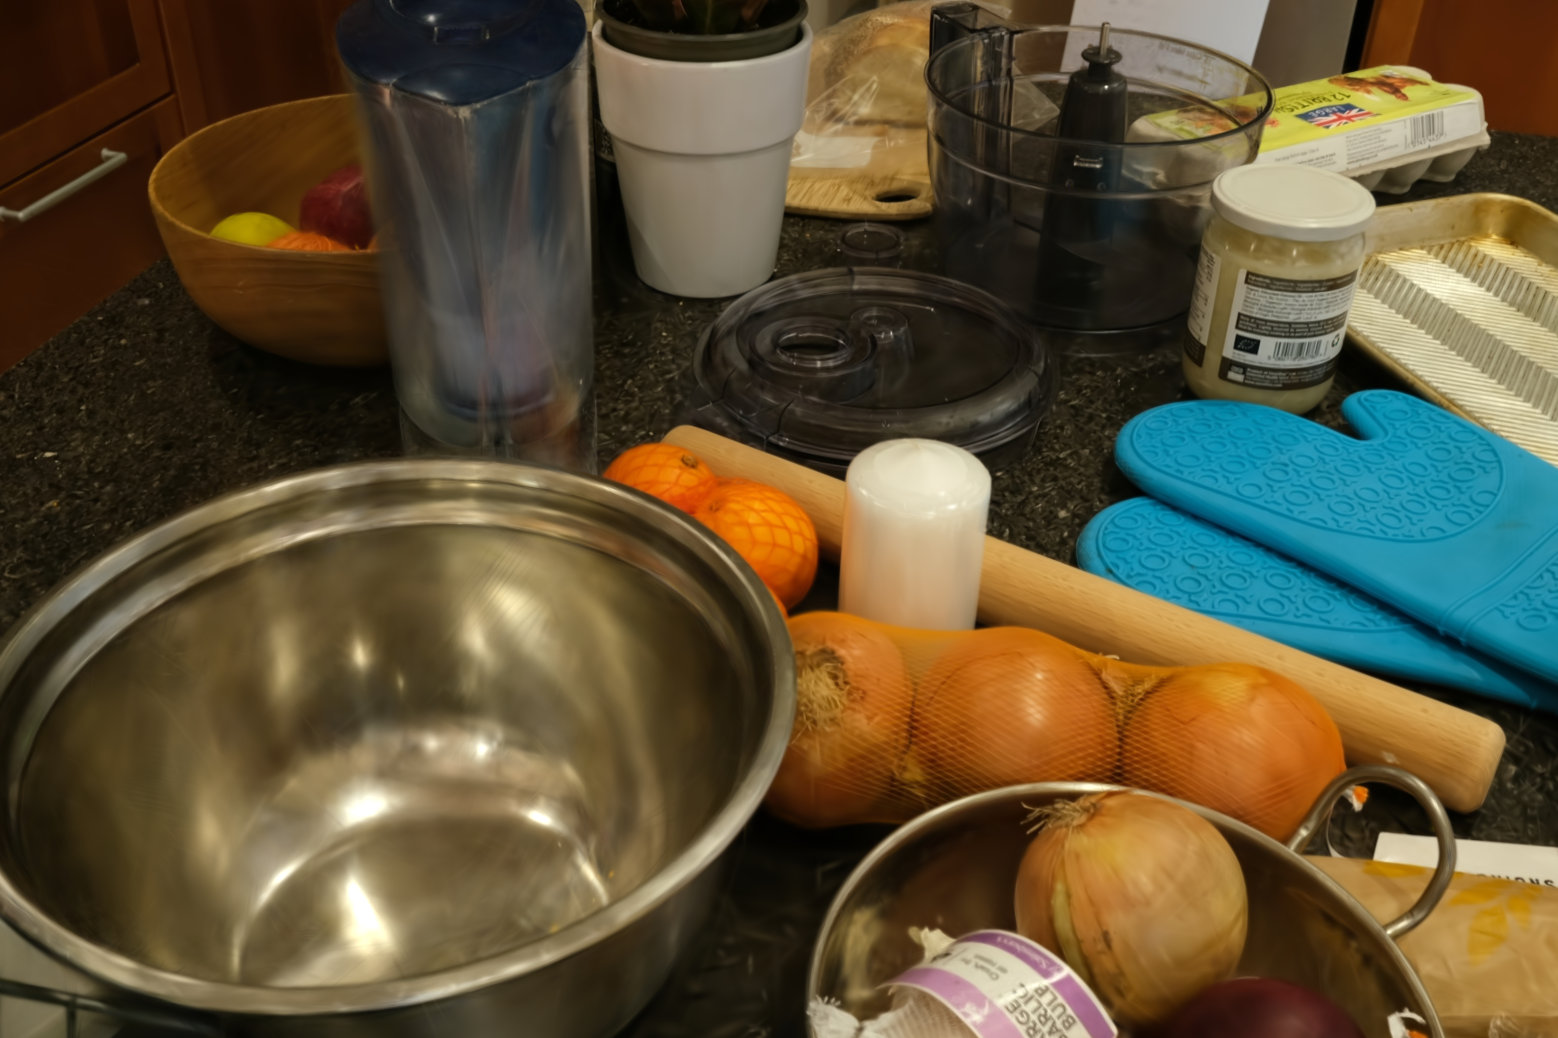
\includegraphics[width=0.3\textwidth]{../o-3dgs/eval/counter/test/ours_30000/renders/00000.png} \\
            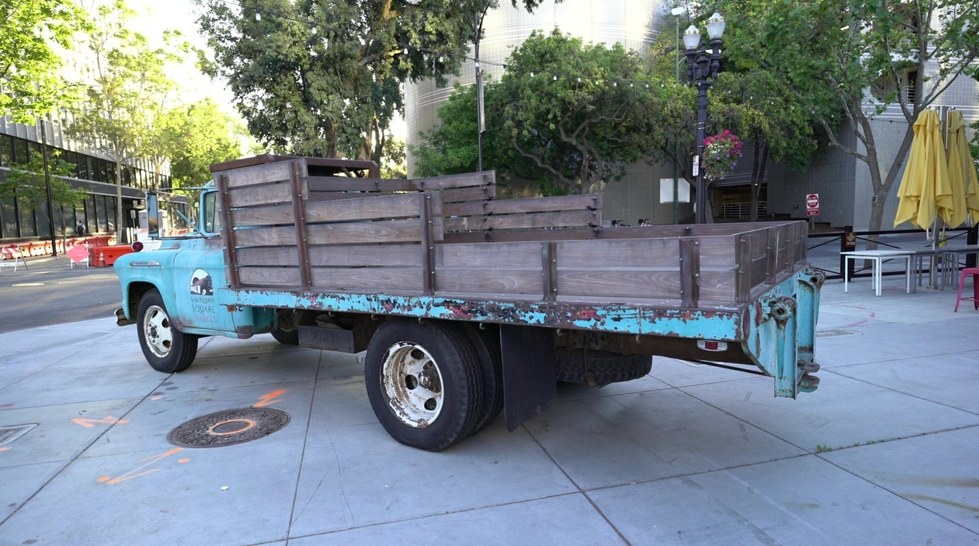
\includegraphics[width=0.3\textwidth]{../o-3dgs/eval/truck/test/ours_30000/gt/00000.png} &
            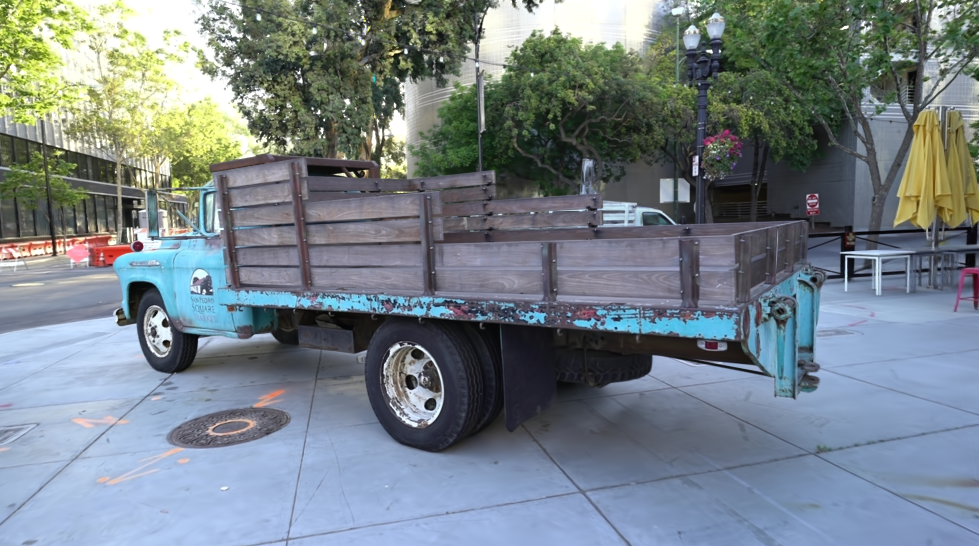
\includegraphics[width=0.3\textwidth]{../o-3dgs/eval/truck/test/ours_30000/renders/00000.png} & 
            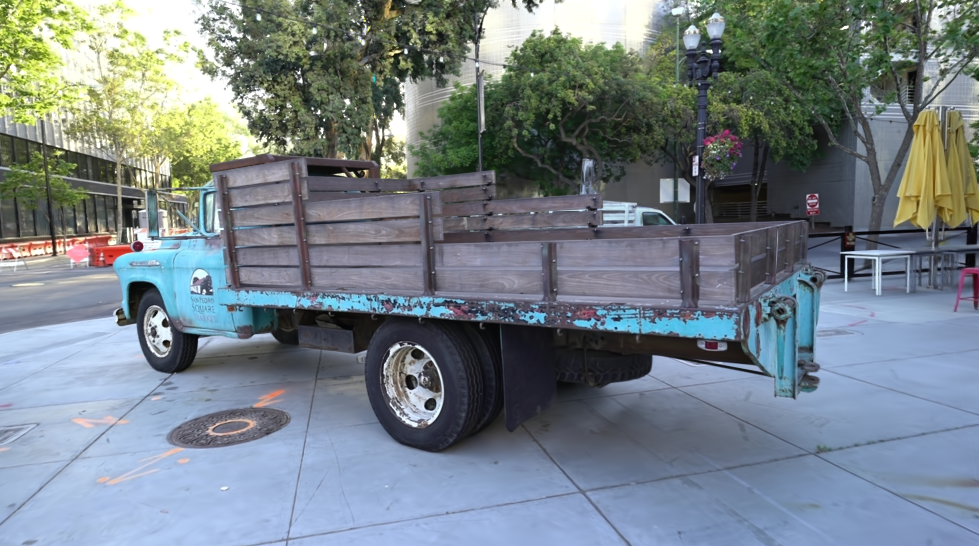
\includegraphics[width=0.3\textwidth]{../o-3dgs/eval/truck/test/ours_30000/renders/00000.png} \\
            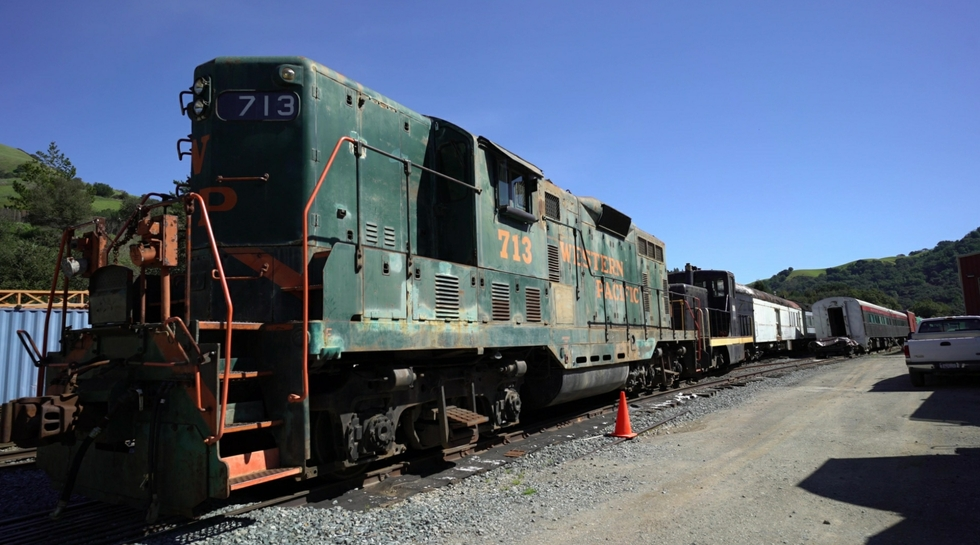
\includegraphics[width=0.3\textwidth]{../o-3dgs/eval/train/test/ours_30000/gt/00000.png} &
            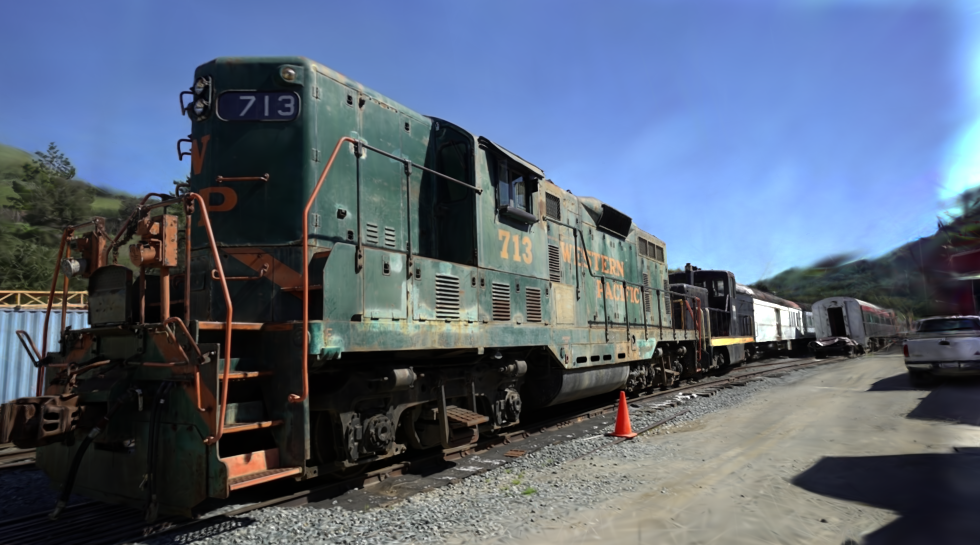
\includegraphics[width=0.3\textwidth]{../o-3dgs/eval/train/test/ours_30000/renders/00000.png} & 
            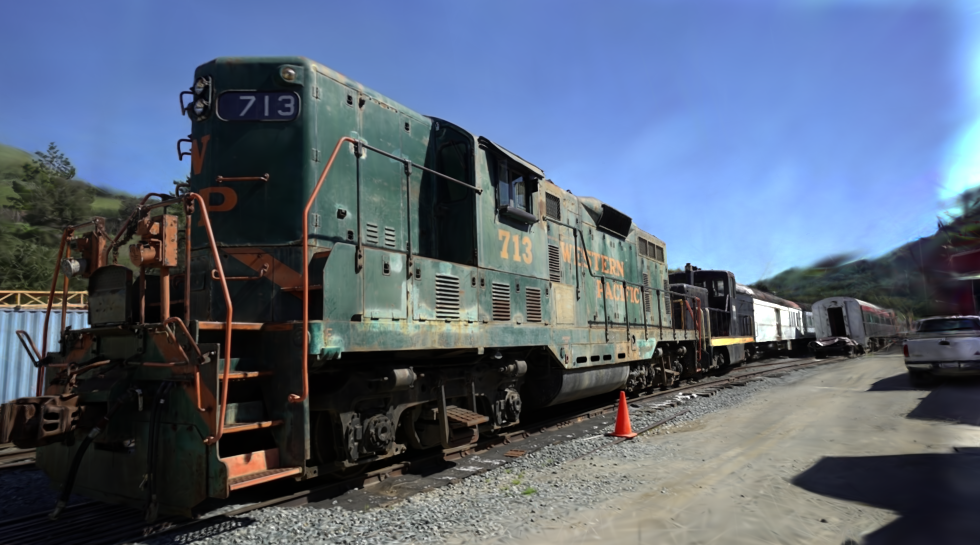
\includegraphics[width=0.3\textwidth]{../o-3dgs/eval/train/test/ours_30000/renders/00000.png} \\
            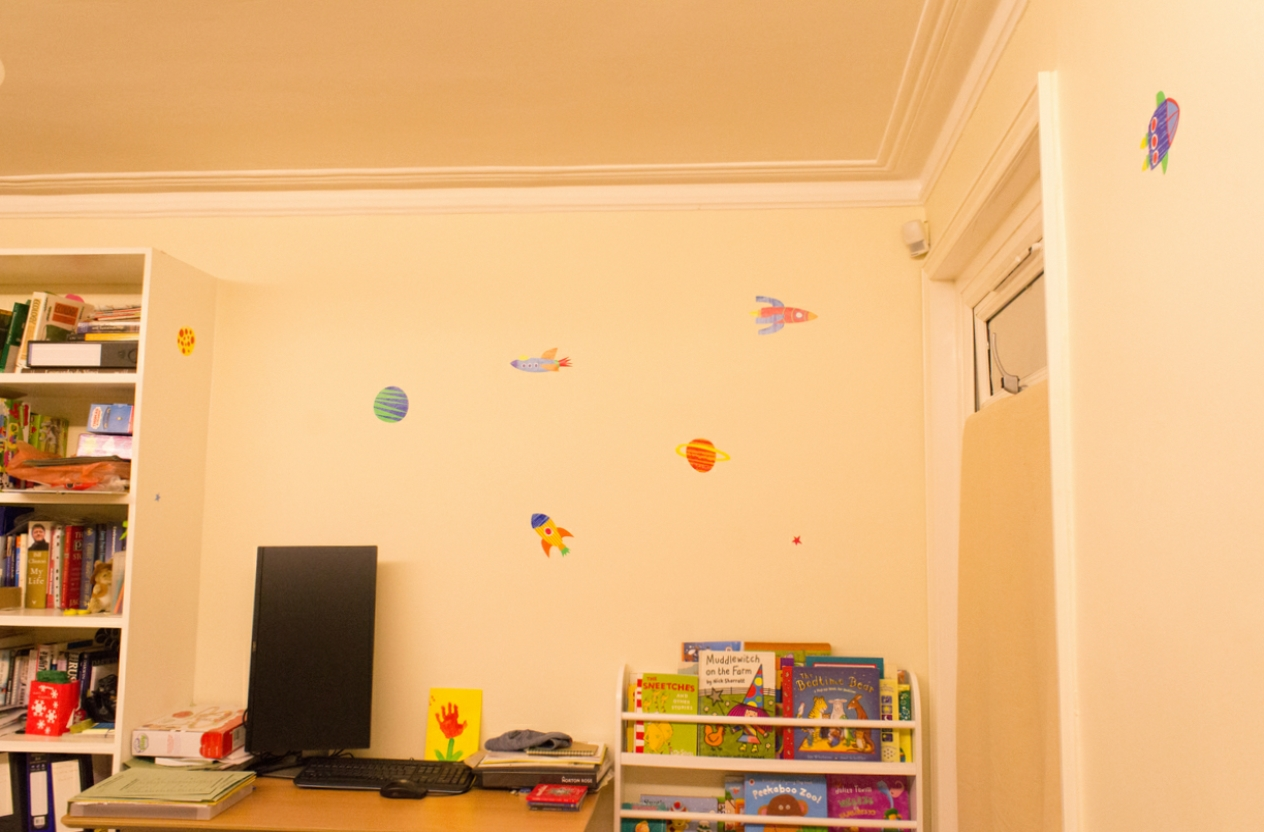
\includegraphics[width=0.3\textwidth]{../o-3dgs/eval/playroom/test/ours_30000/gt/00000.png} &
            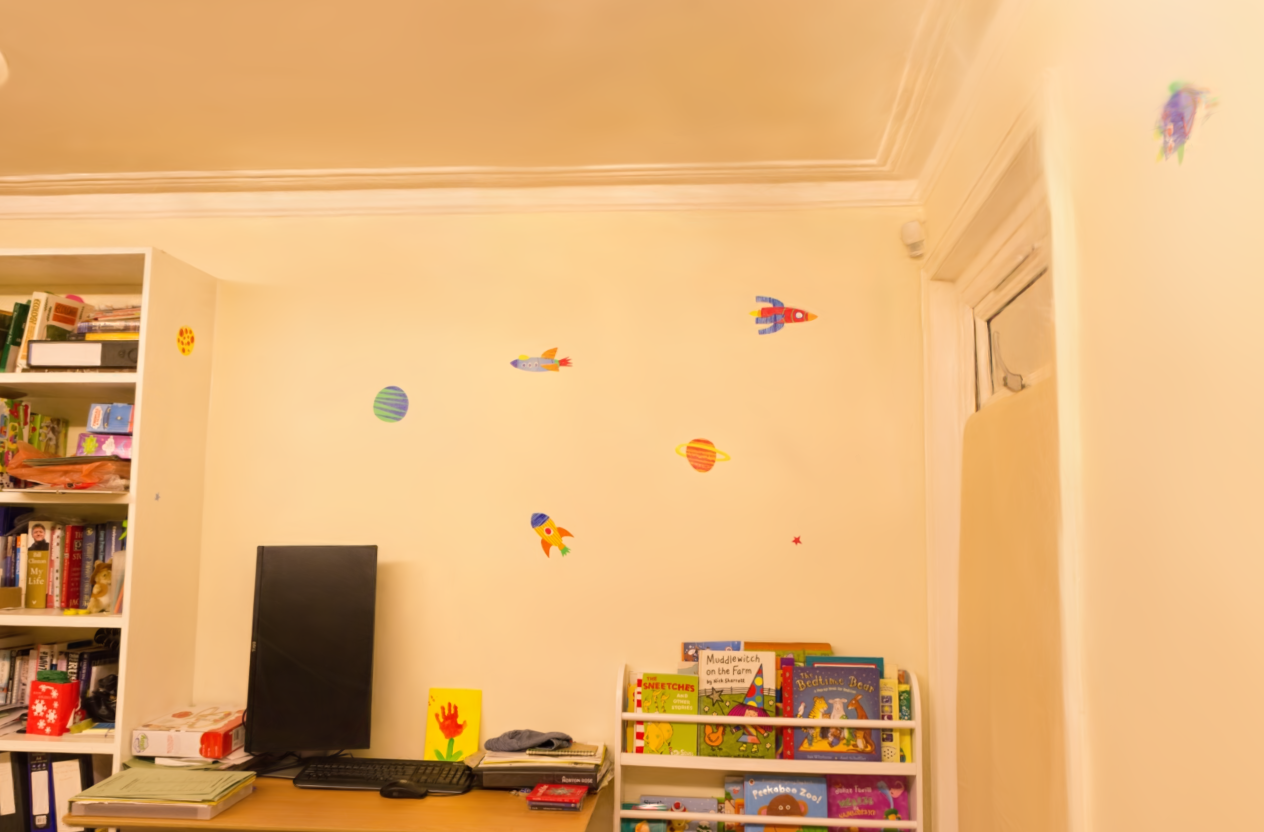
\includegraphics[width=0.3\textwidth]{../o-3dgs/eval/playroom/test/ours_30000/renders/00000.png} & 
            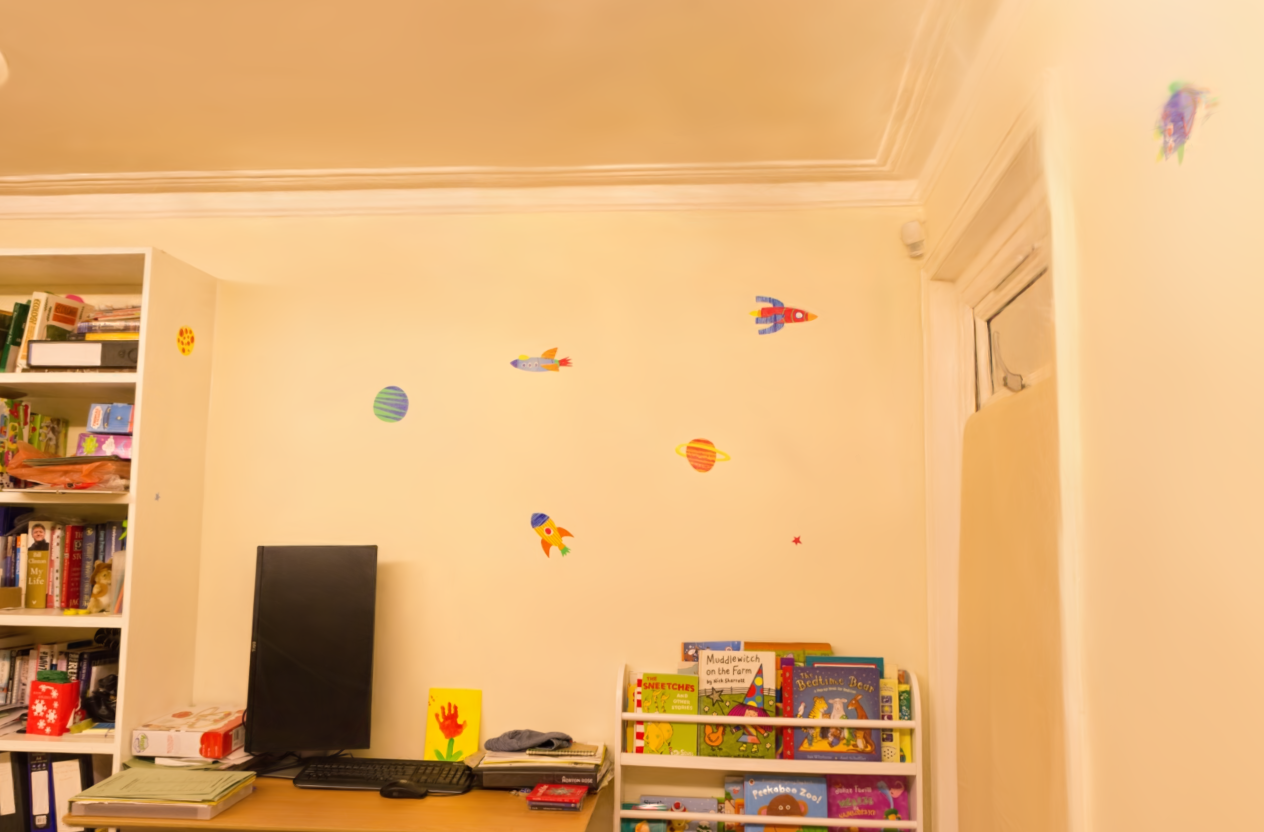
\includegraphics[width=0.3\textwidth]{../o-3dgs/eval/playroom/test/ours_30000/renders/00000.png} \\
            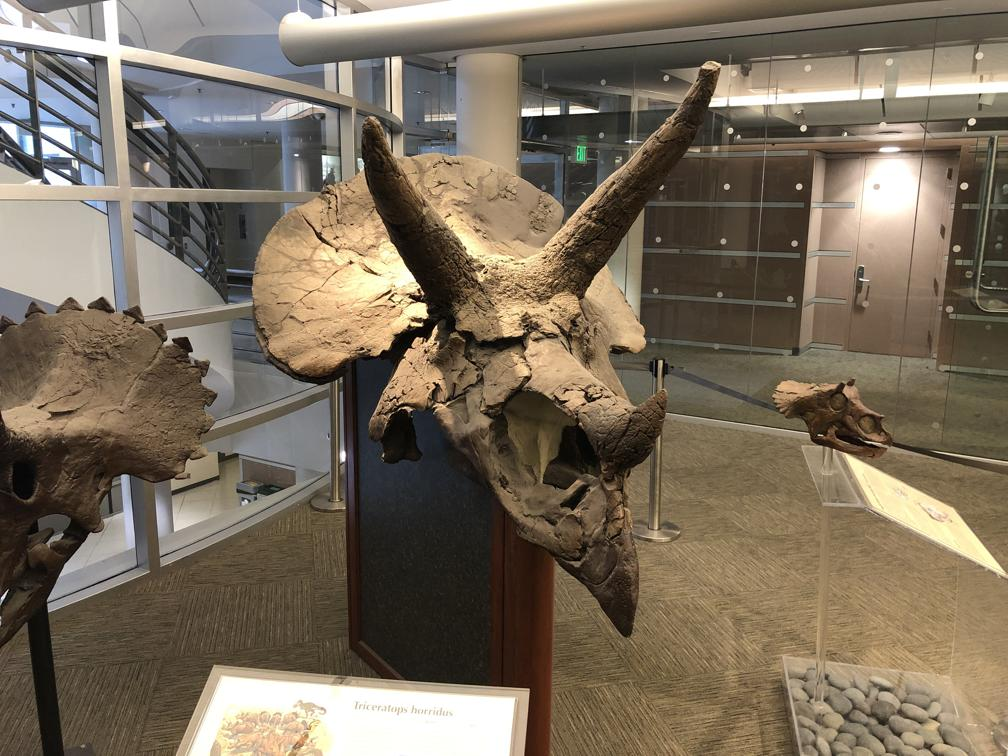
\includegraphics[width=0.3\textwidth]{../o-3dgs/eval/horns/test/ours_30000/gt/00000.png} &
            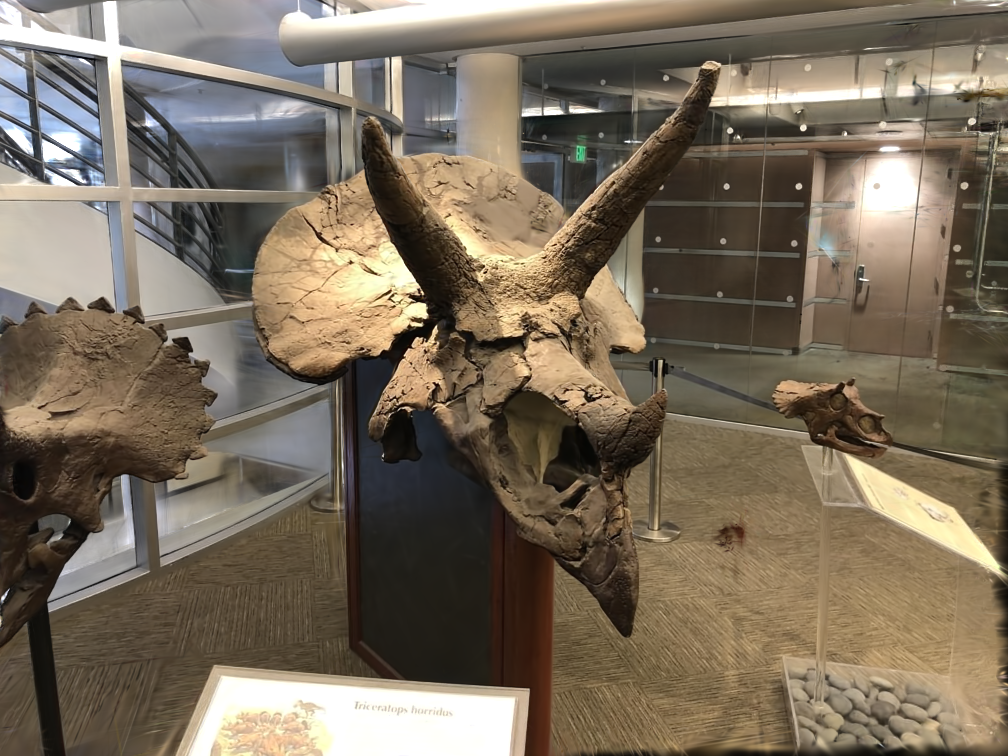
\includegraphics[width=0.3\textwidth]{../o-3dgs/eval/horns/test/ours_30000/renders/00000.png} & 
            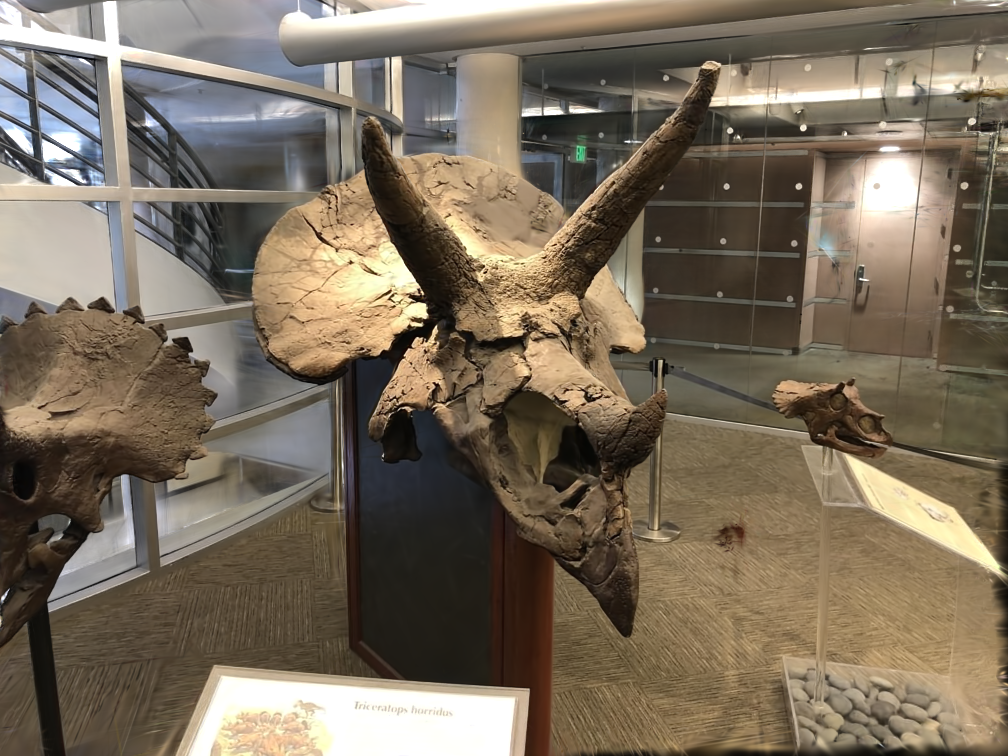
\includegraphics[width=0.3\textwidth]{../o-3dgs/eval/horns/test/ours_30000/renders/00000.png} \\
            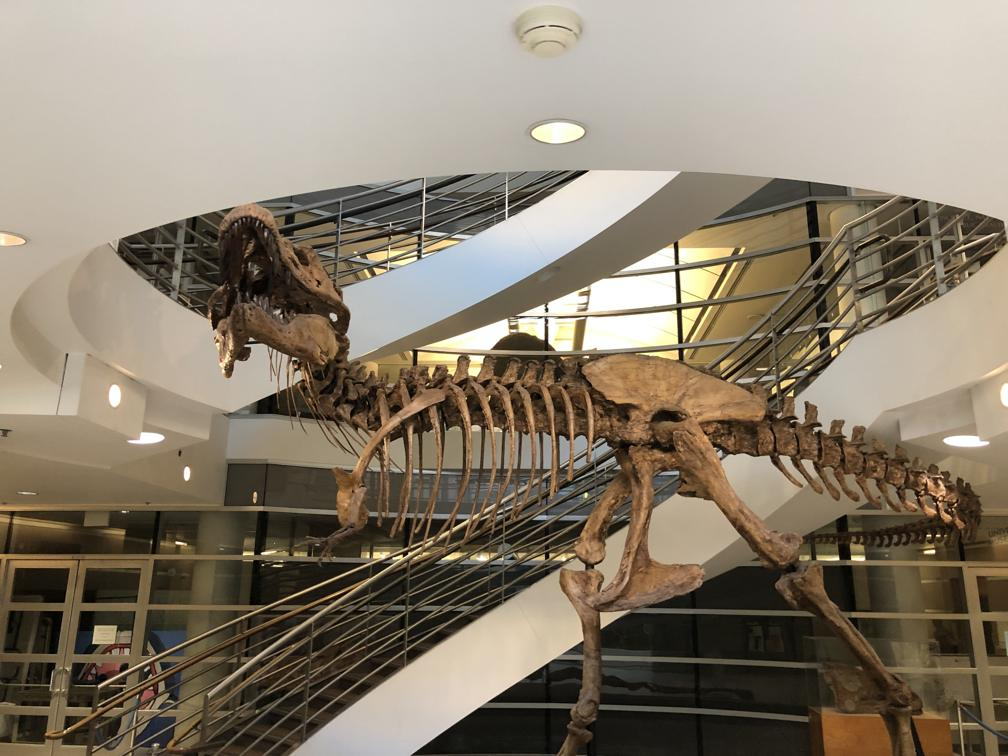
\includegraphics[width=0.3\textwidth]{../o-3dgs/eval/trex/test/ours_30000/gt/00000.png} &
            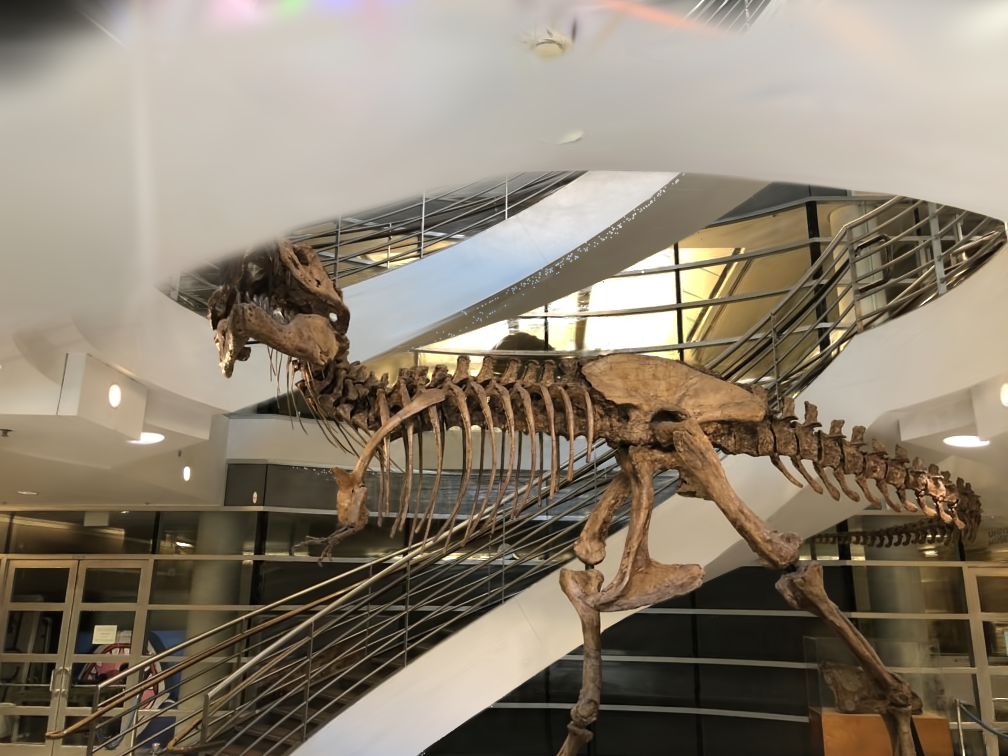
\includegraphics[width=0.3\textwidth]{../o-3dgs/eval/trex/test/ours_30000/renders/00000.png} & 
            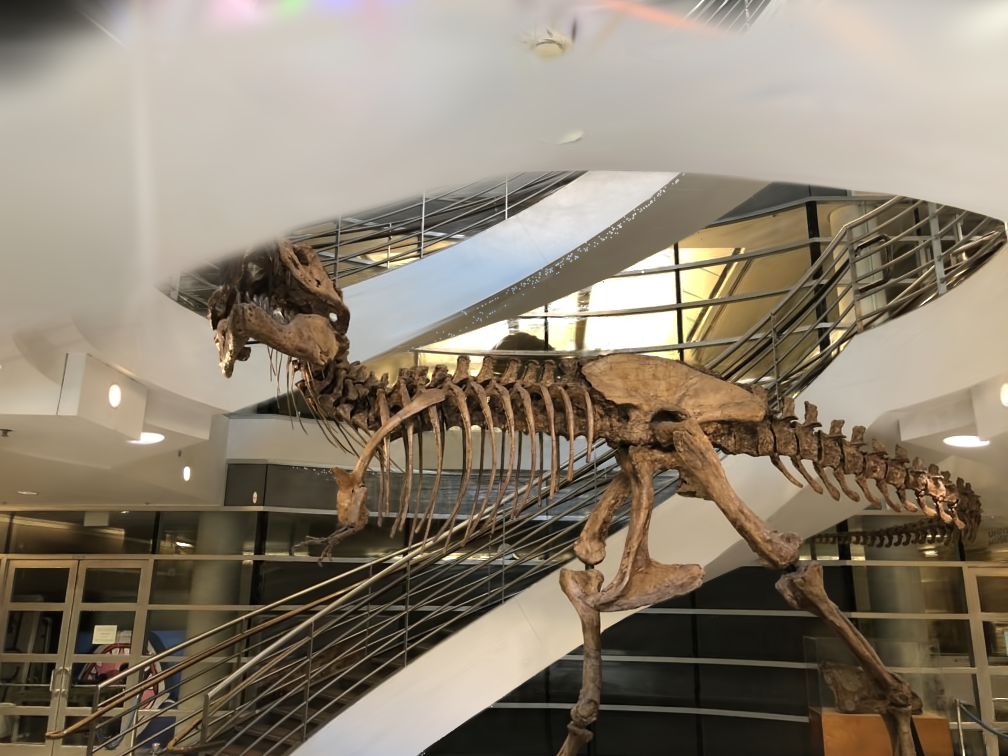
\includegraphics[width=0.3\textwidth]{../o-3dgs/eval/trex/test/ours_30000/renders/00000.png} \\
    \end{tabular}
    
    \caption{Comparison of Ground Truth, 3D-GS, and Ours across different scenes.}
    \label{fig:comparison}
\end{figure}

The qualitative results in Figure~\ref{fig:comparison} demonstrate that the EPO-enhanced model produces sharper and more detailed images compared to the original 3D-GS model. The evolved primitives are better aligned with the geometry and radiance fields, resulting in more accurate and visually appealing renderings.

Several interesting cases highlight different aspects and limitations of our approach. For instance, in the Counter scene from the MipNeRF360 Indoor dataset, our model captures fine details and textures more accurately than the original 3D-GS model. Similarly, in the Train scene from the Tanks and Temples dataset, our method shows improved alignment and detail. However, there are still some limitations. In the Trex scene from the LLFF dataset, our model performs exceptionally well in capturing the fine details of the teeth and ceiling, demonstrating its ability to handle intricate textures and structures. 

These examples illustrate the diversity of datasets and the varying performance of our model across different scenarios. They also highlight the potential for further improvements and optimizations to enhance the scalability and efficiency of our approach.

\section{Quantitative Results}

\begin{table}[htbp]
    \centering
    
    \begin{tabular}{llccccc}
    \toprule
    \textbf{Category} & \textbf{Scene} & \textbf{Method} & \textbf{SSIM$\uparrow$} & \textbf{PSNR$\uparrow$} & \textbf{LPIPS$\downarrow$} & \textbf{Mem} \\
    \midrule
    \multirow{8}{*}{\textbf{MipNeRF360 Indoor}} & 
        \multirow{2}{*}{Counter} 
        & 3D-GS & 0.909 & 29.10 & 0.199 & 255MB \\
            & & \textbf{Our Model} & 0.909 & 29.07 & \textbf{0.198} & 275MB \\
            \cmidrule{2-7} &
        \multirow{2}{*}{Kitchen} 
        & 3D-GS & 0.928 & 31.49 & 0.125 & 378MB \\
            & & \textbf{Our Model} & 0.928 & 31.40 & 0.126 & 393MB \\
            \cmidrule{2-7} &
        \multirow{2}{*}{Bonsai} 
        & 3D-GS & 0.943 & 32.34 & 0.204 & 252MB \\
            & & \textbf{Our Model} & 0.942 & \textbf{32.35} & \textbf{0.203} & 263MB \\
            \cmidrule{2-7} &
        \multirow{2}{*}{Room} 
        & 3D-GS & 0.921 & 31.65 & 0.217 & 309MB \\
            & & \textbf{Our Model} & 0.920 & \textbf{31.66} & \textbf{0.215} & 340MB \\
        \midrule
    \multirow{2}{*}{\textbf{Tanks \& Temples}} & 
        \multirow{2}{*}{Train} 
        & 3D-GS & 0.821 & 22.13 & 0.196 & 257MB \\
            & & \textbf{Our Model} & 0.821 & \textbf{22.19} & 0.197 & 273MB \\
        \midrule
    \multirow{4}{*}{\textbf{LLFF}} & 
        \multirow{2}{*}{Horns} 
        & 3D-GS & 0.887 & 27.21 & 0.132 & 157MB \\
            & & \textbf{Our Model} & 0.887 & \textbf{27.32} & 0.134 & 163MB \\
            \cmidrule{2-7} &
        \multirow{2}{*}{Trex} 
        & 3D-GS & 0.899 & 25.59 & 0.130 & 110MB \\
            & & \textbf{Our Model} & \textbf{0.909} & \textbf{26.66} & \textbf{0.116} & 116MB \\
    \bottomrule
    \end{tabular}
    \caption{Comparison of 3D-GS and Our Model across different scenes and categories. Metrics: SSIM, PSNR, LPIPS, and Memory Usage. Arrows indicate the desired trend for each metric.}
    \label{tab:comparison}
\end{table}
To evaluate the performance of our EPO-enhanced model, we conducted extensive training and testing on the MipNeRF360 Indoor, Tanks and Temples, and LLFF datasets. The results are summarized in Table~\ref{tab:comparison}, 

\chapter{Conclusions and Future Directions}

\section{Conclusions}

The integration of Evolutive Primitive Organization (EPO) into 3D Gaussian Splatting provides a robust solution to the local minima problem. By introducing learnable growing and splitting operations, the algorithm becomes more adaptive and efficient, enhancing the overall performance of 3D rendering models.

In this project, we explored the use of 3D Gaussian Splatting for real-time radiance field rendering. We introduced an adaptive density control mechanism to dynamically adjust the number of Gaussians in the scene, leading to improved representation and rendering quality. Our results demonstrate the effectiveness of this approach in various scenes.

\section{Discussion of Limitations}

While the approach shows promising results, it is still limited by the need for large-scale datasets to train the system effectively. Additionally, the computational cost of the learnable primitives may be high, especially for complex scenes.

While our method shows significant improvements, it has some limitations. The adaptive density control mechanism can be computationally expensive, and the choice of parameters such as the threshold $\epsilon_\alpha$ can significantly impact the results. Additionally, our method may struggle with extremely complex scenes where the number of Gaussians required becomes prohibitively large.

\section{Future Directions}

Future work will explore further optimization of the EPO mechanism, including better training strategies, more efficient backpropagation methods, and applying this technique to a broader range of rendering applications.

Future research could focus on optimizing the adaptive density control mechanism to reduce computational overhead. Exploring alternative representations and hybrid approaches could further enhance the scalability and efficiency of the method. Additionally, investigating the integration of our approach with other neural rendering techniques could lead to even more robust and versatile solutions.

Another promising direction is to explore the possibility of learning the threshold $\epsilon_\alpha$ in the Pruning operation (subsection \ref{subsec:improved_pruning}). Instead of using a fixed heuristic threshold, $\epsilon_\alpha$ could be treated as a learnable parameter that is optimized during training. This would allow the model to dynamically adjust the pruning criteria based on the specific characteristics of the scene and the training objectives, potentially leading to more effective and efficient pruning.

\end{document}